\documentclass[a4paper,11pt,twoside]{scrreport}

\usepackage[lang=de,lib=true]{../general/preamble}

\begin{document}

\makeheaderempty

\begin{titlepage}
    \centering
    Bachelorarbeit Mathematik \\
    \color{DarkBlue}\rule{\linewidth}{1pt}
    \color{Black}\Huge Der Morse-Komplex und Morse-Homologie \\[14pt]
    \color{DarkBlue}\rule{\linewidth}{2pt}
    \color{Black}

    \vspace{3cm}
    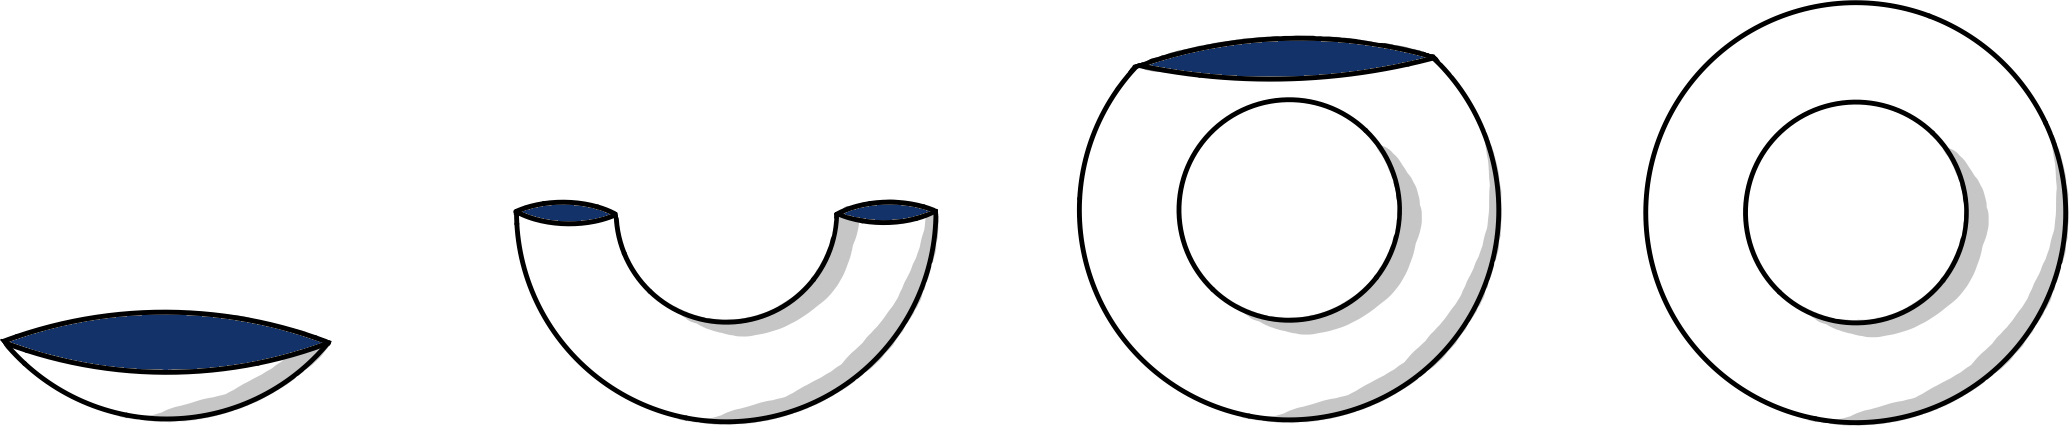
\includegraphics[width=\textwidth]{../resources/Me-Titlepage-Color.jpeg}

    \vfill
    \small

    \textit{eingereicht von}
    \hfill
    \textit{beaufsichtigt von} \\
    Jakob Dimigen
    \hfill
    Prof. Ursula Ludwig

    \vspace{2cm}

    Universität Münster \\
    \vspace{0.02cm}
    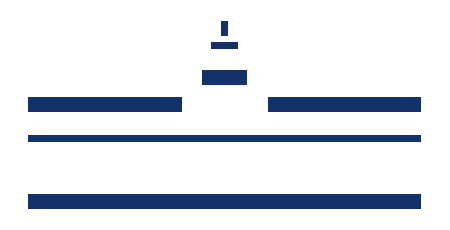
\includegraphics[width=0.2\textwidth]{../resources/WWU_Logo.png}
\end{titlepage}

\section*{Vorwort}

\subsection*{Zielsetzung und Inhalt}

In der Morse Theorie werden glatte Abbildungen $f \colon M \to \R$, deren kritische Punkte 
alle nicht degeneriert sind untersucht. Ein kritischer Punkt ist nicht degeneriert, wenn die Hesseche 
Bilinearform, die lokal durch die Matrix
\[ \left(\pdderive[f]{x_i}{x_j} \right)_{1 \leq i, y \leq n} \]
gegeben ist, nicht ausgeartet ist. Anhand einer solcher Abbildungen lassen sich
Rückschlüsse auf topologische Eigenschaften der Mannigfaltigkeit $M$ ziehen. Das Ziel dieser Arbeit
ist es, den \textit{Morse-Komplex} zu definieren und zu zeigen, dass dieser isomorph zu einem 
zellulären Kettenkomplex ist. Damit ist die \textit{Morse-Homologie}, die Homologie des 
\textit{Morse-Komplexes}, isomorph zur \textit{zellulären Homologie}, die nicht von der gewählten 
zellulären Struktur abhängt. Wir folgen dem ersten Teil des Buches 
\textit{Morse Theory and Fleur Homology} \cite{audin}. 

Im ersten Kapitel wird ein grundlegender Einblick in die Morse-Theorie gegeben. Wichtiges Ergebnis ist
das \textit{Morse-Lemma} das einen konkrete Vorstellung des Verhaltens von Morse-Funktionen in der Nähe 
kritischer Punkte liefert. Weitere wichtige Ergebnisse sind die beiden 
\textit{Deformations-Lemmata}~\ref{satz: erstes deformationslemma} und~\ref{satz: zweites deformationslemma}.

Im zweiten Kapitel untersuchen wir erst die \textit{stabile- und instabile Mannigfaltigkeit} und 
definieren den \textit{Raum der Trajektorien}. Die Trajektorien sind Flüsse von eines Pseudo-Gradientenfeldes.
Diese starten und enden immer in kritischen Punkten. Das $k$-te Glied des Morse-Komplexes ist dann dasjenige
$\F_2$-Modul, das von den kritischen Punkten mit Index $k$ erzeugt wird, und das differenzial ist gegeben
durch die Anzahl der Trajektorien von kritischen Punkten mit Index $k$ zu kritischen Punkten mit Index 
$k - 1$. Wir zeigen, dass dieser Komplex wohldefiniert ist und dass es ein Kettenkomplex ist. 

Im dritten Kapitel wird bewiesen, dass der Morse-Komplex isomorph zum einem zellulären Komplex ist. 
Dann werden einige Anwendungen der Morse-Homologie gegeben.

\subsection*{Geschichte der Morse Theorie}

Die Morse-Theorie ist zu Ehren des amerikanischen Mathematikers \textit{Marston Morse} benannt, der
grundlegende Ergebnisse zum Beispiel wie das \textit{Morse-Lemma}~\ref{satz: morse-lemma} in 
\cite{morse} schon im Jahre 1929 bewies. In den späten 60er Jahren untersuchte dann 
bewies.

\subsection*{Vorraussetzungen}

Wir setzen vorraus, dass der Leser sich mit Mannigfaltigkeiten auskennt. Außerdem sollten 
grundlegende Begriffe der Topologie wie \textit{Homotopie}, \textit{Homotopietyp} ... \todo{...}
bekannt sein. Weiterhin sollten Grundlagen der homologischen Algebra bekannt sein, also 
Definitionen von \textit{Kettenkomplex} und \textit{Homologie}.

\subsection*{Notation}

Folgende Notationen werden benutzt:

\begin{itemize}
    \item $\isom$ für eine Vektorraum-Isomorphie oder eine Homeomorphie.
    \item $\diffeo$ für einen Diffeomorphismus.
    \item Die Tangentialräume werden immer als die Menge der Derivationen betrachtet.
    \item Um Subskripte in Subskripten weitestgehend zu vermeiden, ist ein Vektorfeld eine 
        glatte Abbildung $X \colon M \to TM$ mit $p \mapsto X(p) \in T_pM$ (anstatt $X_p$).
    \item ist $f \colon M \to \N$ eine glatte Abbiildung, dann ist die Tangentialabbildung
        von $f$ im Punkt $p$ die Abbildung $\opd f (p) \colon T_pM \to T_{f(p)}N$.
\end{itemize}

\tableofcontents

\chapter{Morse-Funktionen und Pseudo-Gradienten}

\makeheaderfancy
\setcounter{page}{1}

In diesem Kapitel beschäftigen wir uns näher mit den Stars dieser Arbeit: \\
\textit{Morse-Funktionen} und \textit{Pseudo-Gradientenfeldern}. Außerdem werden wir das 
\textit{Morse-\\Lemma}~\ref{satz: morse-lemma} und die so genannten 
\textit{Deformations-Lemmata}~\ref{satz: erstes deformationslemma} und~\ref{satz: zweites deformationslemma} 
beweisen, die allein von den kritischen Punkten einer Morse Funktion 
Rückschlüsse auf die topologischen Eigenschaften der Mannigfaltigkeit zulassen.

\section{Nicht-Degeneriertheit und Index}

Dieser Abschnitt folgt dem ersten Kapitel aus \cite{milnor}. Wir werden Grundlegende Begriffe der
Morse-Theorie erklären und das \textit{Morse-Lemma}~\ref{satz: morse-lemma} beweisen.

\begin{definition}[Kritischer Punkt]
    \label{def: kritischer Punkt}
    Sei $M$ eine glatte Mannigfaltigkeit und $f \colon M \to \R$ eine glatte Abbildung. 
    Ein \textit{kritischer Punkt} von $f$ ist ein Punkt $p \in M$, sodass $\opd f (p)$ nicht 
    surjektiv ist.
    Die Menge der kritischen Punkte von $f$ heißt $\Crit (f)$. Ist $p$ ein kritischer Punkt, dann
    heißt $f(p)$ kritischer Wert von $f$.
\end{definition}

\begin{remark}
    Wir werden uns ausschließlich mit glatten Abbildungen $f \colon M \to \R$ beschäftigen.
    bei solchen Abbildungen ist $p \in M$ ein kritischer Punkt genau dann, wenn 
    $\opd f (p) = 0$.
\end{remark}

Wir würden gerne eine Hessesche Bilinearform für die Tangentialräume der Mannigfaltigkeit
definieren, allerdings ist dies ein nicht ganz einfaches Unterfangen. Wir werden am Ende
einen Begriff erhalten, der mit dem der gewohnten Hesseschen Bilinearform im $\R^n$
übereinstimmt, allerdings nur für kritische Werte definiert ist.

\begin{definition}[Hessesche Bilinearform]
    Es sei $f \colon M \to \R$ eine glatte Abbildung, $p$ ein kritischer Punkt von $f$.
    Es seien $x, y \in T_pM$. Wähle $X, Y \in \VFs (M)$, sodass $X(p) = x$ und 
    $Y(p) = y$. Definiere nun
    \[ \opd^2 f (x, y) (p) = X(p)(Y(\cdot)f). \]
    $\opd^2 f (\cdot, \cdot) (p)$ heißt \textit{Hessesche Bilinearform}. 
\end{definition}

\begin{prop}
    \label{prop: hessesche ist sym bilinearform}
    $\opd^2 f (\cdot, \cdot) (p)$ hängt nicht von den gewählten Vektorfeldern $X$ und $Y$ ab 
    und ist für alle kritischen Punkte eine symmetrische Bilinearform.
\end{prop}

\begin{proof}
    Wir betrachten die so genannte \textit{Lie-Klammer} für Vektorfelder $X$ und $Y$:
    \[ [X, Y] = XY - YX , \]
    wobei
    \[ (XY - YX) (p) (f) = X(p)(Y(\cdot)(f)) - Y(p)(X(\cdot)(f)) . \]
    Man rechnet nach, dass die Lie-Klammer symmetrisch ist und das für jeden kritischen Punkt $p$
    von $f$ gilt $[X, Y](p)(f) = 0$.
    Bilinearität folgt dann direkt aus der Definition. Da $p$ ein kritischer Punkt ist gilt 
    \[ \opd^2 f (x, y) (p) - \opd^2 f (y, x) (p) = [X, Y] (p) (f) = 0, \]
    die Zuordnung ist also symmetrisch. Außerdem gilt
    \[ XY f (p) = X(p) (Y(\cdot) f) = x(Y(\cdot) f), \]
    also hängt die Form nicht von $X$ ab, und wegen der Symmetrie auch nicht von $Y$.
\end{proof}

\begin{definition}[nicht-degeneriert, Index]
    \label{def: nicht-degeneriert u index}
    Es sei $f \colon M \to \R$ eine glatte Abbildung, $p$ ein kritischer Punkt von
    $f$. Wir nennen $p$ \textit{nicht degeneriert}, falls die Bilinearform 
    $\opd^2 f (\cdot, \cdot) (p)$ nicht ausgeartet ist. Der \textit{Index} eines
    nicht degenerierten kritischen Punktes $p$ ist die maximale Dimension $\Index (p)$ der
    Untervektorräume, auf denen $\opd^2 f (\cdot, \cdot) (p)$ negativ definit ist.
    Die Menge der kritischen Punkte von $f$ mit Index $k$ heißt $\Crit_k (f)$.
\end{definition}

\begin{remark}
    Nicht-Degeneriertheit und Index lassen sich auch über lokale Koordinaten definieren.
    Tatsächlich stimmt die Sichtweise über lokale Koordinaten mit der Vorstellung der Hesseschen-
    Bilinearform, die wir für Abbildungen $\R^n \to \R$ haben überein:

    Es seien $\phi = (x_1, ..., x_n)$ lokale Koordinaten um den kritischen Punkt $p$. 
    Dann ist $\mathcal{B} = \left(\pderive{x_1}, ..., \pderive{x_n}\right)$ eine Basis des
    Vektorraums $T_pM$. Wir bekommen
    \[ 
        \opd^2 f \left( \pderive{x_i}, \pderive{x_j} \right) (p) 
        = \pderive{x_i}(p) \left( \pderive[f]{x_j} \right) 
        = \pdderive[f]{x_j}{x_i} (p).
    \]
    Dann ist $p$ nicht degeneriert genau dann wenn die Matrix
    \[ H^\phi_p(f) = \left( \pdderive[f]{x_i}{x_j} \right)_{1 \leq i, j \leq n} \]
    invertierbar ist. Der Index von $p$ ist dann die Anzahl der negativen Eigenwerte
    von $H^\phi_p(f)$. Der Index und die nicht-degeneriertheit hängen offensichtlich
    nicht von den gewählten Koordinaten ab, aber die Matrix $H_p^{\phi}(f)$ schon.
\end{remark}

Die beiden Begriffe Index und nicht-Degeneriertheit sind zentral in der Morse-Theorie 
und werden uns über die gesamte Arbeit begleiten. Auch der nachfolgende Satz wird in 
fast jedem Beweis genutzt:

\begin{theorem}[Morse-Lemma]
    \label{satz: morse-lemma}
    Es sei $p$ ein nicht degenerierter kritischer Punkt mit Index $k$ einer glatten 
    Funktion $f \colon M \to \R$. Dann existieren lokale Koordinaten 
    $\phi = (x_1, ..., x_n)$, sodass in einer Umgebung $U$ von $p$ gilt:
    \[ f = f(p) - x_1^2 - ... - x_k^2 + x_{k + 1}^2 + ... + x_n^2
        \; \text{ und } \;
        \varphi (p) = 0 . \]
    $(U, \phi)$ heißt \textit{Morse-Karte}, und $U$ \textit{Morse-Umgebung}.
\end{theorem}

Der hier geführte Beweis für das Morse-Lemma ist in \cite{hirsch} zu finden. 
Bevor wir das Morse Lemma beweisen, benötigen wir eine Aussage aus der Linearen Algebra:

\begin{lemma}
    \label{lemma: lina lemma}
    Es sei $A = \diag(a_1, ..., a_n)$ eine diagonale $n \times n$ Matrix mit 
    Diagonaleinträgen $\pm 1$. Dann gibt es eine Umgebung $N$ von $A$ im Vektorraum der 
    symmetrischen $n \times n$ Matrizen und eine glatte Abbildung 
    $P \colon N \to GL_n(\R)$, sodass $P(A) = E_n$ und falls $P(B) = Q$, dann gilt 
    $Q^TBQ = A$.
\end{lemma}

\begin{proof}
    Die Aussage kann man Induktiv über $n$ beweisen, siehe \cite{hirsch}.
\end{proof}

\begin{proof}[Beweis von Satz~\ref{satz: morse-lemma}]
    Es sei $U$ eine Karten Umgebung von $p$. Dann können wir ohne Beschränkung der 
    Allgemeinheit annehmen, dass $f \colon \R^n \to \R$, $p = 0$ und $f(0) = 0$.
    Außerdem können wir mithilfe eines Korrdinatenwechsels annehmen, dass $A := H_0(f)$
    eine Diagonalmatrix mit ausschließlich Diagonaleinträgen $\pm 1$ ist, denn da $p$
    nicht degeneriert ist ist $A$ invertierbar. 
    \begin{claim*}
        Es existiert eine glatte Abbildung $x \mapsto B_x$ von $M$ in die symmetrischen
        $n \times n$ Matrizen, sodass für $B_x = (b_{ij}(x))_{ij}$ gilt 
        \[ f(x) = \sum_{i, j = 1}^n b_{ij}(x) x_i x_j , \]
        und sodass $B_0 = A$. 
    \end{claim*}
    \begin{smallproof}
        Da $f(0) = 0$ bekommen wir mit dem Fundamentalsatz der 
        Differenzial - und Integralrechnung: 
        \begin{align*}
            f(x) = & f(x) - f(0) 
                = \int_0^1 \derive[f (tx)]{t} \opd t \\
            = & \int_0^1 \sum_{i = 1}^n \pderive[f]{x_i}(tx) x_i \opd t 
                = \sum_{i = 1}^n \left( \int_0^1 \pderive[f]{x_i}(tx) \opd t \right) x_i ,
        \end{align*}
        Denn da $p = 0$ ein kritischer Punkt ist, gilt $\pderive[f]{x_i}(0) = 0$ für alle 
        $i$. Mit dem selben Argument sehen wir dann, dass
        \[ \pderive[f]{x_i}(tx) = 
        \sum_{j = 1}^n \left( \int_0^1 \pdderive[f]{x_i}{x_j}(stx) \opd s \right) x_j . \]
        Dann gilt 
        \[ f(x) = 
            \sum_{i, j = 1}^n 
            \left( \int_0^1 \int_0^1 \pdderive[f]{x_i}{x_j} (x) \opd s \opd t \right) 
            x_i x_j 
        . \]
        Setze also 
        \[ b_{ij}(x) = \int_0^1 \int_0^1 \pdderive[f]{x_i}{x_j} (x) \opd s \opd t . \]
        Dann gilt schon $B_0  = A$, und die Abbilfungen $b_{ij}$ sind glatt, also 
        auch $x \mapsto B_ x$.
    \end{smallproof}
    Wir dürfen nun das vorherige Lemma~\ref{lemma: lina lemma} anwenden:

    Sei $P \colon N \to GL_n(\R)$ eine Abbildung wie in~\ref{lemma: lina lemma}.
    Setze $Q_x := P(B_x)$. Definiere nun eine glatte Abbildung $\phi \colon U \to \R^n$
    durch $\phi (x) = Q_x^{-1}x$ in einer Umgebung von $0$. Wir rechnen nach, dass 
    $\opd \phi (0) \colon \R^n \to \R^n$ die Identität ist:

    Schreibe $Q_x^{-1} = (q_{ij}(x))_{ij}$. Dann
    \[ \phi(x) = \left( 
        \sum_{k = 1}^n q_{1k}(x) x_k, \cdots , \sum_{k = 1}^n q_{nk}(x) x_k
        \right)
    \]
    Also 
    \begin{align*}
        \pderive[\phi_i]{x_j} (x) 
            = & \pderive{x_j} \left( \sum_{k = 1}^n q_{ik} (x) x_k \right) \\
        = & \sum_{k = 1}^n \left( 
            \pderive[q_{ik}]{x_j}(x) x_k + q_{ik}(x) \delta_{ki}
        \right)
    , \end{align*}
    Wobei $\delta_{ki}$ das Kronecker Delta ist. Setzen wir also $0$ ein
    bekommen wir
    \[ \pderive[\phi_i]{x_j}(0) = q_{ij}(0). \]
    Das Differential von $\phi$ in $0$ ist also gegeben durch
    \[ Q_0^{-1} = P(B_0)^{-1} = P(A)^{-1} = E_n . \]
    Das Differential an der Stelle $0$ ist also invertierbar, und dann können wir mit dem 
    Satz über die Umkehrfunktion annehmen, dass $U$ klein genug ist, sodass $\phi$ 
    eingeschräkt aufs Bild ein Diffeomorphismus ist. 
    Dann ist $\phi$ eine Karte um $0$. Setze $(y_1, ..., y_n) := \phi$, dann gilt 
    \begin{align*}
        f(x) = & x^T B_x x 
            = (Q_x \phi(x))^T B_x (Q_x \phi(x)) \\
        = & \phi(x)^T (Q_x^T B_x Q_x) \phi(x) 
            = \phi(x)^T A \phi(x) \\
        = & \sum_{i = 1}^n a_{ii} y_i(x)^2
    . \end{align*}
    Das entspricht genau der gewünschten Form, denn $a_{ii} \in \{ \pm 1 \}$.
\end{proof}

\begin{corollary}
    Jeder nicht degenerierte kritische Punkt besitzt eine offene Umgebung, in der sich keine weiteren
    kritischen Punkte befinden.
\end{corollary}

\section{Morse-Funktionen}

In diesem Abschnitt untersuchen wir \textit{Morse-Funktionen}:

\begin{definition}[Morse-Funktion]
    \label{satz: morse-funktion}
    Eine \textit{Morse-Funktion} auf einer glatten Mannigfaltigkeit $M$ ist eine glatte Funktion
    $f \colon M \to \R$, deren kritische Punkte alle nicht degeneriert sind.
\end{definition}

Insbesondere sehen wir, dass Morse-Funktionen allgegenwertig sind. Dafür zeigen wir, dass für 
eine Untermannigfaltigkeit $M \subseteq \R^n$ und einen Punkt $p \in \R^n$ die Abbildung
$x \mapsto \| x - p \|^2$ nur für $p$, die so gennanten \textit{Brennpunkte}
sind, keine Morse Funktion ist, und dass die Menge der Brennpunkte eine Nullmenge ist. Dann werden
wir sehen, dass jede glatte Funktion (auf gewisse Art und Weise) beliebig nah an einer Morse 
Funktion ist. Dieser Abschnitt folgt zu großen Teilen \cite{milnor} und \cite{audin}.

\begin{example}
    \label{bsp: morse funktion}
    Ein Paar Beispiele:
    \begin{enumerate}
        \item Die Höhenfunktion auf dem Torus, die wir am Anfang dieses Kapitels untersucht haben, ist 
            ein Beispiel für eine Morse-Funktion.
        \item Ist $T = [0, 1]^2 / \sim$ wie üblich der Torus, dann ist $f \colon T \to \R$ mit 
            $f(x, y) = -\cos(\pi \cdot x) + -\cos(\pi \cdot y)$ eine Morse Funktion. 
            \begin{figure}[H]
                \centering
                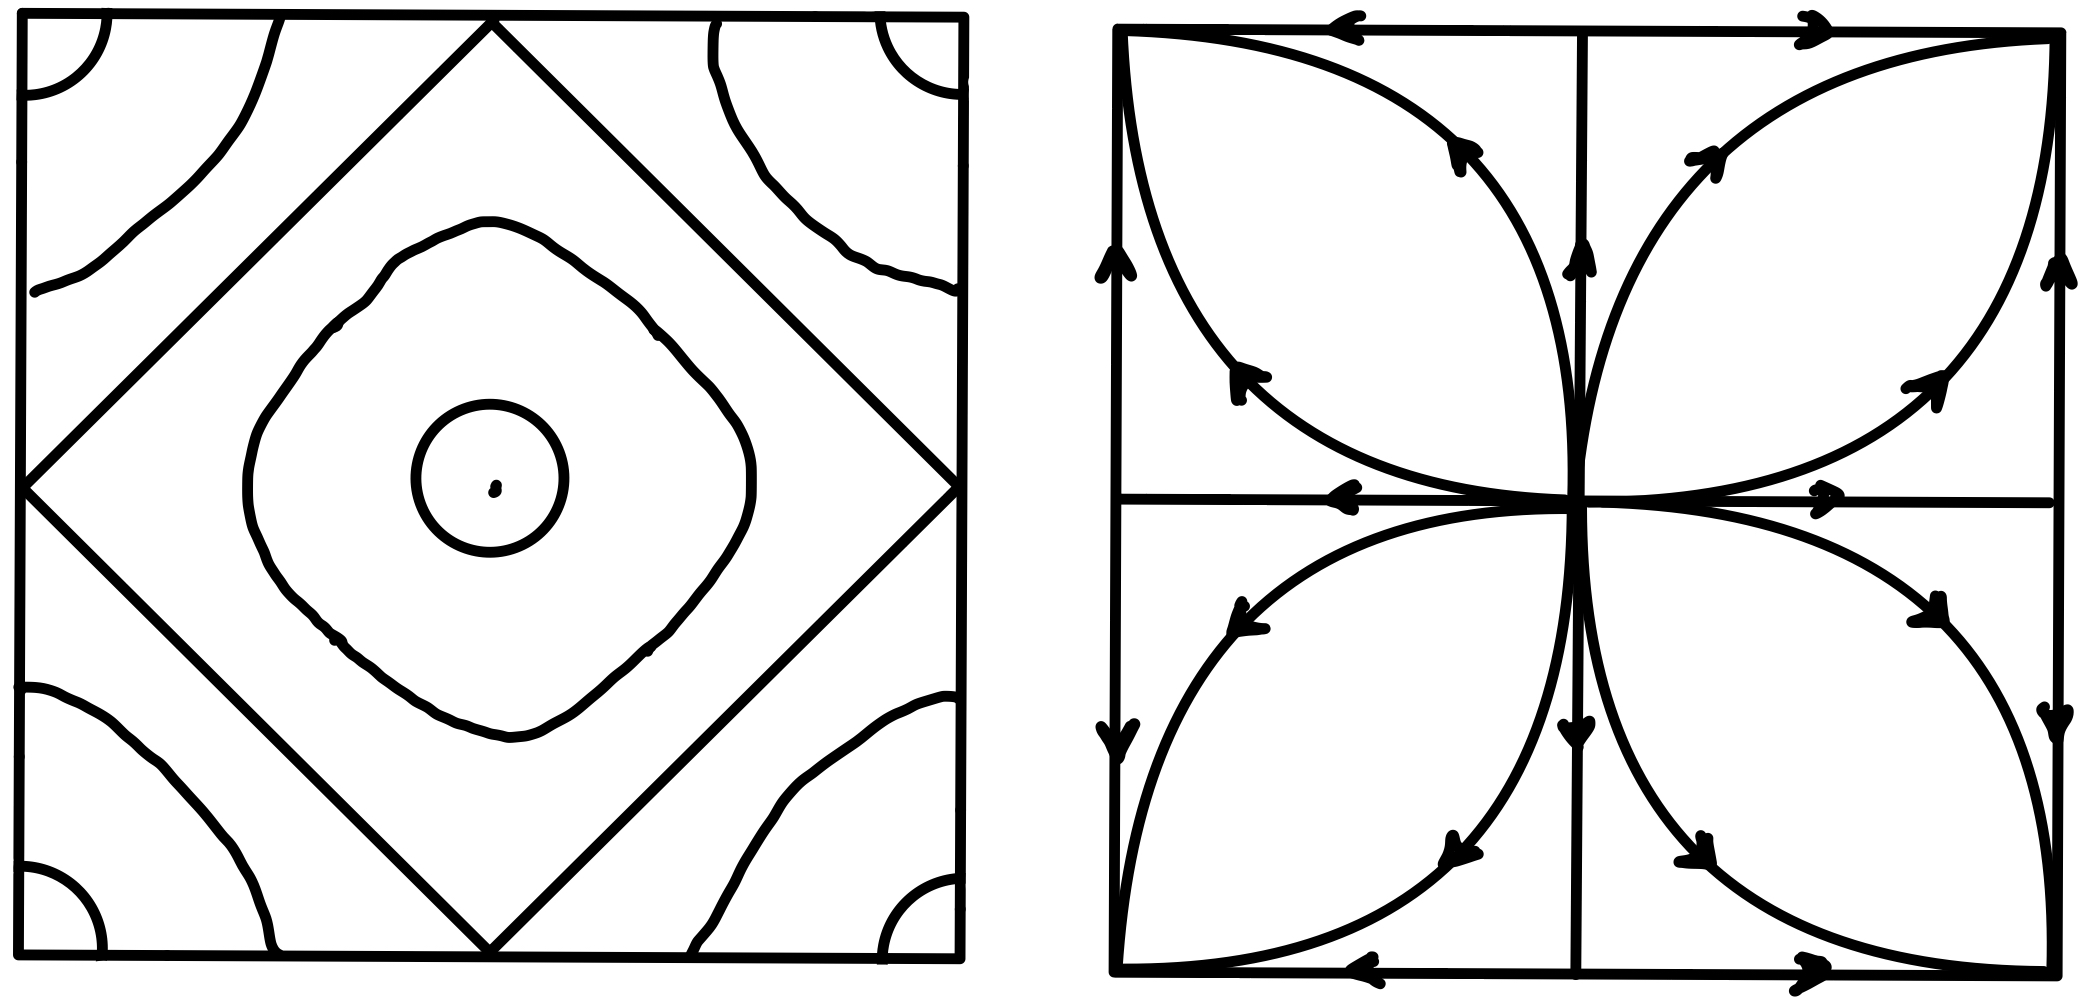
\includegraphics[width=0.4\textwidth]{../resources/morse-funktion-torus.jpeg}
                \caption{Höhenlinien (links) und der Gradient (rechts) von $f$}
            \end{figure}
    \end{enumerate}
\end{example}

\begin{definition}[Normalenbündel]
    \label{def: normalenbuendel}
    Es sei $M \subseteq \R^n$ eine Untermannigfaltigkeit von $\R^n$. Das Normalenbündel ist die 
    Menge
    \[ NM = \{ (x, v) \in M \times \R^n : v \perp T_xM \} . \]
    Wir betrachten hier $T_xM \subseteq T_x\R^n \isom \R^n$ via der Basis 
    $\left( \del / \del x_i \right)$, wobei $x_i$ die Achsen des $\R^n$ sind.
\end{definition}

\begin{prop}
    \label{prop: NM ist untermannigfaltigkeit}
    Das Normalenbündel $NM$ ist eine $n$-dimensionale Untermannigfaltigkeit von $M \times \R^n$.
\end{prop}

\begin{proof}
    Es sei $x \in M$. Dann existiert eine Umgebung $U \subseteq \R^n$ von $x$, eine Umgebung 
    $\Omega \subseteq \R^d$ von $0$ und eine Einbettung 
    \begin{align*}
        h \colon \Omega \longto & \R^n \\
        (u_1, \dots, u_d) \; \longmapsto & \; x(u_1, \dots, u_d)
    \end{align*}
    die ein Diffeomorphismus $h \colon \Omega \to U \cap M$ ist. Das orthogonale Komplement 
    von $T_xM$ in $\R^n$ hat Dimension $n - d$. Es sei also 
    $(v_1(x), ..., v_{n-d}(x))$ eine Basis von $(T_xM)^{\perp}$. Dann ist 
    \[ (u_1, ..., u_d, t_1, ..., t_{n - d}) \longmapsto 
        \left(x(u_1, ..., u_n), \sum_{k = 1}^{n - d} t_k \cdot v_k(u_1, ..., u_d)\right) \]
    eine lokale Parametrisierung von $NM$ als Untermannigfaltigkeit von $M \times \R^n$.
\end{proof}

\begin{definition}[Brennpunkt]
    \label{def: brennpunkt}
    Es sei $M \subseteq \R^n$ eine Untermannigfaltigkeit von $\R^n$. Es sei $E \colon NM \to R^n$ 
    mit $E (x, v) = x + v$. Ein \textit{Brennpunkt} von $M$ ist ein kriticher Wert von $E$.
\end{definition}

\begin{remark}
    Aus dem Satz von Sard (siehe \cite{sard}) folgt, dass die Menge der Brennpunkte eine 
    Nullmenge ist. Intuitiv sind die Brennpunkte einer Untermannigfaltigkeit die Punkte im 
    $\R^n$, an denen sich die Normalen von nahe aneinanderliegenden Punkten schneiden.
\end{remark}

Brennpunkte und das Normalenbündel werden hier nur für den Beweis von 
Proposition~\ref{prop: existenz morse-funktionen} genutzt, geben aber eine schöne Intuition.

\begin{lemma}
    \label{lemma: char. von Brennpunkten}
    Es sei $M \subseteq \R^n$ eine Untermannigfaltigkeit, $x \in M$ und $NM$ parametriesiert wie im 
    Beweis von Proposition~\ref{prop: NM ist untermannigfaltigkeit}. Dann ist $p = x + v$ genau 
    dann ein Brennpunkt von $M$, wenn die Matrix 
    \[
        \left( \left\langle \pderive[x]{u_j}, \pderive[x]{u_i} \right\rangle - 
        \left\langle v , \pdderive[x]{u_i}{u_j} \right\rangle \right)_{ij}
    \]
    nicht invertierbar ist.
\end{lemma}

\begin{proof}
    Den Beweis findet man zum Beispiel bei Milnor in Kapitel 6 von \cite{milnor}.
\end{proof}

\begin{prop}
    \label{prop: existenz morse-funktionen}
    Es sei $M \subseteq \R^n$ eine Untermannigfaltikgeit. Für fast jeden Punkt in $\R^n$ ist
    die Funktion
    \begin{align*}
        f_p \colon M & \longrightarrow \R \\
        x & \longmapsto \| x - p \|^2
    \end{align*}
    eine Morse-Funktion.
\end{prop}

\begin{proof}
    Offensichtlich ist $f_p$ glatt. Das Differential von $f_p$ erweitert auf $\R^n$ mit 
    derselben Vorschrift ist
    \[ \opd f_p (x) = 2 (x - p). \]
    Also gilt
    \[ \opd f_p (x) (v) = \langle 2 (x - p), v \rangle . \]
    $x \in M$ ist folglich genau dann ein kritischer Punkt von $f_p$, wenn $T_xM$ orthogonal 
    zu $(x - p)$ ist.

    Bemerke, dass für eine Abbildung $f \colon \R^n \to \R$ mit $f = \langle \phi_1, \phi_2 \rangle$,
    $\phi_1, \phi_2 \colon \R^n \to \R^n$ und eine Derivation $X_p$ gilt 
    \[ X_p (f) = \langle X_p(\phi_1), \phi_2 \rangle + \langle \phi_1, X_p(\phi_2) \rangle.  \]
    Sei nun $x \in M$. Dann existiert eine Umgebung $U \subseteq \R^n$ von $x$, eine Umgebung 
    $\Omega \subseteq \R^d$ von $0$ und eine Einbettung 
    \[ h \colon \Omega \longto \R^n , \]
    mit $h \colon \Omega \to U \cap M$.
    Schreibe
    \[ h(u_1, ..., u_n) = x(u_1, ..., u_n). \]
    Dann bekommen wir die partiellen Ableitungen
    \[ 
        \pderive[f_p]{u_i} = \sum_{k = 1}^n \pderive[f_p]{x_k} \cdot \pderive[x_k]{u_i} 
        = \left\langle 2(x - p), \pderive[x]{u_i} \right\rangle 
    \]
    und 
    \[ 
        \pdderive[f_p]{u_i}{u_j} = 
            2 \left( \left\langle \pderive[x]{u_j}, \pderive[x]{u_i} \right\rangle + 
            \left\langle x - p , \pdderive[x]{u_i}{u_j} \right\rangle \right) 
    . \]
    
    Also hat nach Lemma~\ref{lemma: char. von Brennpunkten} $f_p$ in einer Umgebung von $x$ genau 
    dann nicht-degenerierte kritische Punkte, wenn $f_p$ ein Brennpunkt von $M$ ist. Mit der 
    Bemerkung nach der Definition von Brennpunkten~\ref{def: brennpunkt} folgt dann direkt die 
    Behauptung.
\end{proof}

\begin{remark}
    Mit dem Einbettungssatz von Whitney (siehe \cite{whitney}) folgt dann direkt, dass es auf 
    jeder Mannigfaltigkeit $M$ viele Morse-Funktionen gibt. Es gilt sogar noch eine stärkere 
    Aussage:
\end{remark}

\begin{prop}
    \label{prop: morse-approximation}
    Es sei $M$ eine Mannigfaltigkeit, $f \colon M \to \R$ glatt. Dann kann $f$ in jeder kompakten
    Teilmenge $K$ beliebig gut von einer Morse Funktion approximirt werden, also für jedes 
    $\eps > 0$ existiert eine Morse Funktion $g \colon K \to \R$, sodass 
    \[ \| \, f - g \, \|_{\infty} < \eps . \]
\end{prop}

\begin{proof}
    Den Beweis findet man bei Audin und Damian in \cite{audin}.
\end{proof}

Die meiste Zeit werden wir uns in dieser Arbeit kompakte Mannigfaltigkeiten untersuchen,
auf solchen kann jede glatte Funktion sogar global mit einer Morse Funktion approximieren.

\section{Vektorfelder und Pseudo-Gradienten}

Wir untersuchen erst ein paar Eigenschaften von Vektorfeldern.

\begin{definition}[Flusslinie]
    \label{def: flussliene}
    Es sei $I \subseteq \R$ ein Intervall, $M$ eine glatte Mannigfaltigkeit und  
    $\gamma \colon I  \to M$ ein glatter Weg. Dann definiere für $t_0 \in \R$
    \[ \derive[\gamma]{t} (t_0) := 
        \opd \gamma (t_0) \left( \pderive{t} \right) \in T_{\gamma(t_0)}M \]
    wobei $\pderive{t}$ das von der Identität auf $\R$ induzierte Element in $T_t\R$ ist.

    Es sei $X \in \VFs (M)$ ein Vektorfeld auf $M$. $\gamma$ heißt Flusslinie von $X$,
    falls für alle $t_0 \in \R$ gilt: 
    \[ \derive[\gamma]{t}(t_0) = X(\gamma(t_0)) . \]
    Das Bild einer Flusslinie von $X$ heißt \textit{Trajektorie}. Wir benutzen den Begriff 
    Trajektorie recht frei. Manchmal ist damit auch die Flusslinie gemeint.
\end{definition}

\begin{definition}[1-Parameter Gruppe aus Diffeomorphismen]
    \label{def: 1-parameter gruppe aus diffeos}
    Es sei $M$ eine glatte Mannigfaltigkeit. Eine 
    \textit{1-Parameter Gruppe aus Diffeomorphismen} ist eine glatte Abbildung
    \begin{align*}
        \phi \colon \R \times M \longto & \; M \\
        (t, p) \longmapsto & \; \phi_t(p)
    \end{align*}
    sodass gelten: 
    \begin{itemize}
        \item Für alle $s, t \in \R$ gilt $\phi_{s + t} = \phi_s \circ \phi_t$ und
        \item $\phi_0 = \id_{M}$.
    \end{itemize}

    Für eine 1-Parameter Gruppe aus Diffeomorphismen $\phi$ schreiben wir 
    \[ \varphi_{\bullet}(p): \R \to M ; t \mapsto \varphi_t(p) . \]

    Es sei $X \in \VFs (M)$. Eine 1-Parameter Gruppe aus Diffeomorphismen $\phi$ heißt 
    \textit{von $X$ erzeugt}, falls für alle $p \in M$ gilt:
    \[ X(p) = \derive[\phi_{\bullet}(p)]{t}(0) \]
\end{definition}

\begin{remark}
    Wie der Name suggeriert, ist für jedes $t \in \R$ die Abbildung $\phi_t$ ein 
    Diffeomorphismus: Das Inverse von $\phi_t$ ist $\phi_{-t}$.

    Ist außerdem $\phi$ eine von einem Vektorfeld $X$ erzeugte 1-Parameter Gruppe aus 
    Diffeomorphismen, dann rechnet man leicht nach, dass $\phi_{\bullet}(p)$ Flusslinien 
    von $X$ sind.
\end{remark}

\begin{prop}
    \label{prop: kompaktes VF generiert 1-param. grp.}
    Es sei $M$ eine glatte Mannigfaltigkeit, $X \in \VFs (M)$ mit kompaktem Träger. Dann 
    generiert $X$ eine eindeutige 1-Parameter Gruppe aus Diffeomorphismen.
\end{prop}

\begin{proof}
    Einen Beweis für diese Aussage findet man zum Beispiel auch in \cite{milnor}.
\end{proof}

\begin{remark}
    Falls $M$ eine kompakte Mannigfaltigkeit ist, dann generieren alle Vektorfelder eindeutige 
    1-Parametergruppen aus Diffeomorphismen.
\end{remark}

% \begin{definition}[Riemannsche Metrik]
%     \label{def: riemannsche metrik}
%     Es sei $M$ eine Mannigfaltigkeit. Es sei 
%     \[ g_p \colon T_pM \times T_pM \longto T_pM \]
%     ein Skalarprodukt für jedes $p \in M$, sodass für alle $X, Y \in \VFs (M)$ die Abbildung 
%     \[ p \longmapsto g_p(X(p), Y(p)) \]
%     glatt ist. Dann heißt $g$ \textit{Riemmannsche Metrik} auf $M$. Wir schreiben für 
%     $x, y \in T_pM$ 
%     \[ \langle x, y \rangle := g_p(x, y) \text{ und } \| x \| := \sqrt{g_p(x, x)} . \]
% \end{definition}

% \begin{remark}
%     Man kann zeigen, dass alle Mannigfaltigkeiten eine Riemannsche Metrik besitzen.
% \end{remark}

% \begin{definition}[Gradient]
%     \label{def: gradient}
%     Es sei $M$ eine glatte Mannigfaltigkeit, $f \colon M \to \R$ eine glatte Abbilding. Dann 
%     ist der Gradient von $f$ das eindeutige Vektorfeld $\grad f$, sodass für alle $X \in \VFs (M)$
%     gilt 
%     \[ \langle X , \grad f \rangle = \opd f X . \]
% \end{definition}

\begin{definition}[Pseudo-Gradient]
    \label{def: pseudo-gradient}
    Es sei $M$ eine Mannigfaltigkeit, $f \colon M \to \R$ eine glatte Funktion. $X \in \VFs (M)$
    heißt \textit{Pseudo-Gradient} oder \textit{Pseudo-Gradientenfeld} von $f$, falls gelten:
    \begin{itemize}
        \item $\opd f (p) (X(p)) \leq 0$ für alle $p \in M$, mit Gleichheit genau dann wenn 
            $p$ ein kritischer Punkt von $f$ ist.
        \item Für jeden kritischen Punkt $p$ von $f$ existiert eine Morse-Umgebung 
            $(U_p, \phi_p)$, in der $X (q) = 
                - \opd (\phi_p^{-1}) (q) \cdot \grad (f \circ \phi_p^{-1})$.
    \end{itemize}
    $\grad$ ist hier der Standardgradient auf $\R^n$, der vom Standardskalarprodukt auf $\R^n$ 
    induziert wird.
\end{definition}

Die erste Eigenschaft haben auch Gradientenfelder. Tatsächlich ist dies die einzige
Eigenschaft des Gradienten, die uns in diesem Kontext interessiert.

Die zweite Eigenschaft stellt sicher, dass sich Pseudo-Gradientenfelder in der nähe von 
kritischen Punkten, also den Punkten, die wir in dieser Arbeit untersuchen, einfach verhält, 
nämlich genau wie durch das Morse-Lemma~\ref{satz: morse-lemma} bestimmt.

\begin{prop}
    Es sei $M$ eine Mannigfaltigkeit und $f \colon M \to \R$ eine Morse-Funktion. 
    Dann existiert ein Pseudo-Gradientenfeld von $f$.
\end{prop}

\begin{proof}
    Den Beweis findet man bei Audin und Damian \cite{audin}.
\end{proof}
\section{Topologische Eigenschaften anhand kritischer Punkte}
\label{sec: topologische eigenschaften anhand kritischer punkte}

Wir wollen die beiden Deformations-Lemmata beweisen, die eine Verbindung zwischen den topologischen
Eingeschaften einer Mannigfaltigkeit und den kritischen Punkten einer Morse Funktion herstellt.
Ist $f \colon M \to \R$ eine glatte Abbildung, dann ist die Subniveaumenge von $f$ bezüglich 
einer reellen Zahl $c$ die Menge $M^c := f^{-1}(- \infty, c]$. Sind $a < b$ reelle Zahlen, dann
stellen die Deformationslemmata die Topologien von $M^a$ und $M^b$ in Relation: Das erste beschreibt, 
was passiert \textit{wenn kein} kritischer Wert überschritten wird, und das zweite beschreibt, was 
passiert \textit{wenn ein} kritischer Wert überschritten wird. Die Beweise folgen Milnors Buch 
\cite{morse}. \\

\begin{theorem}[Erstes Deformationslemma]
    \label{satz: erstes deformationslemma}
    Es sei $M$ eine glatte Mannigfaltigkeit und $f: M \rightarrow \R$ eine
    glatte Abbildung. Hat $f$ keine kritischen Werte im Intervall $[a, b]$ und 
    ist $f^{-1}[a, b]$ kompakt, so existiert ein Diffeomorphismus 
    $M^b \rightarrow M^a$, und $M^a$ ist ein Deformationsretrakt von $M^b$.
\end{theorem}

Die Idee des Beweises ist es, $M^b$ entlang eines Pseudo-Gradientenfeldes von $f$ mit einem 
Diffeomorphismus $\varphi$ "nach unten zu ziehen", bis $\varphi(f^{-1}(b)) = f^{-1}(a)$.

\begin{proof}
    Sei $Y$ ein Pseudo-Gradientenfeld von $f$. Es existiert eine kompakte Umgebung $K \in M$ von 
    $f^{-1}[a, b]$, in der keine kritischen Punkte enthalten sind, das folgt zum Beispiel aus 
    Whitneys Einbettungssatz und dem Satz von Heine-Borel. Sei $\rho: M \to \R$ eine glatte, 
    positive Funktion, sodass
    \[ \rho(p) = - \frac{1}{\opd f (p) (Y (p))} \]
    für alle $p \in f^{-1}[b, a]$ und die außerhalb von $K$ verschwindet und für
    die für alle $p \in K$, die keine kritischen Punkte sind, gilt: 
    \[ 0 \leq \rho(p) \leq - \frac{1}{\opd f (p) (Y (p))} . \]
    Bemerke dass $\rho$ innerhalb von $K$ wohldefiniert ist, da sich keine kritischen Punkte in $K$ 
    befinden. Definiere ein Vektorfeld $X$ durch
    \[ X(p) = \rho(p) \cdot Y (p) \]
    Dann hat $X$ kompakten Träger, erfüllt also die Vorraussetzungen von 
    Lemma~\ref{prop: kompaktes VF generiert 1-param. grp.}. Sei also $\varphi$ die
    einzigartige 1-Parameter Gruppe aus Diffeomorphismen, die von $X$ generiert
    wird. 
    Wir bekommen für jedes $p \in M$ eine Abbildung 
    $f \circ \varphi_{\bullet}(p): \R \to \R$.
    
    \begin{claim*} 
        Für alle $p \in M$, $t_0 \in \R$ und $q = \varphi_{t_0}(q)$
        ist $\derive{t} f \circ \varphi_{\bullet}(p) (t_0) \in [-1, 0]$ und falls 
        $f(\varphi_t(q)) \in [a, b]$ gilt sogar $\derive{t} f \circ \varphi_{\bullet}(q) (t_0) = -1$.
    \end{claim*}

    \begin{smallproof}
        Für $q = \varphi_{t_0}(p)$:
        \begin{align*}
            \derive{t} f \circ \varphi_{t_0}(p)
            & = \opd f (\varphi_{t_0}(p)) \cdot \opd \varphi_{\bullet}(p) (t_0) 
                \left( \derive{t} \right)
            = \opd f (q) ( X(q) ) \in [-1, 0]
        \end{align*}
        $f \circ \varphi_{\bullet}(p)$ ist also monoton wachsend für alle $p \in M$.
        Falls sogar $f(\varphi_p(t_0)) \in [b, a]$, dann gilt
        \[ \frac{d}{dt} f \circ \varphi^p (t_0) = -1 \]
    \end{smallproof}

    Man zeigt dann leicht, dass für $p \in f^{-1}(b)$, $t_0 \in [0, b - a]$ gilt 
    $f(\varphi_{t_0}(p)) \in [b, a]$.

    Dann ist für $p \in f^{-1}(b)$ die Abbildung $f \circ \phi_{\bullet}(p)$ im Intervall $
    [0, b - a]$ linear mit Steigung $- 1$ und es gilt 

    \[ f(\varphi_{b - a}(p)) = f(\varphi_{0}(p)) + (b - a) = b \]
    Genauso für $q \in f^{-1}(b)$: $f(\varphi_{a - b}(q)) = a$, also 
    $\varphi_{b - a}(f^{-1}(a)) = f^{-1}(b)$.

    Dann haben wir $\varphi_{b - a} (M^b) = M^a$, also ist $\varphi_{b - a}|_{M^b}$ ein 
    Diffeomorphismus zwischen $M^a$ und $M^b$. 

    Betrachte nun $r: M^b \times \R \to M^a$,
    \[  
        r(p, t) = \begin{cases}
            p & \text{ falls }  f(p) \leq a \\
            \varphi_{t(f(p) - a)}(p) & \text{ falls } a \leq f(p) \leq b 
        \end{cases}
    \]

    $r$ ist stetig, $r(\cdot, 0)$ ist die Identität auf $M^b$, $r(\cdot, 1)|_{M^a}$ ist die 
    Identität auf $M^a$ und \\ $r(1, M^b) \subseteq M^a$, also ist $M^a$ ein Deformationsretrakt 
    von 
    $M^b$.
\end{proof}

\begin{theorem}[Zweites Deformations-Lemma]
    \label{satz: zweites deformationslemma}
    Es sei $M$ eine glatte Mannigfaltigkeit, $f: M \rightarrow \R$ eine glatte
    Abbildung und $p$ ein nicht-degenerierter kritischer Punkt mit Index 
    $k$. Sei $c := f(p)$ und $\varepsilon \geq 0$, sd. 
    $f^{-1}[c - \varepsilon, c + \varepsilon]$ kompakt ist und außer $p$ keine 
    weiteren kritischen Punkte von $f$ beinhaltet. Dann hat $M^{c-\varepsilon}$
    denselben Homotopietypen wie $M^{c - \varepsilon} \cup e^k$.
\end{theorem}

\begin{proof}
    Die Idee für den Beweis ist, sich eine neue Funktion $F: M \to \R$ zu definieren,
    die Außerhalb von einer kleinen Umgebung von $p$ $f$ entspricht und in der 
    Umgebung etwas kleiner ist. Dann bekommen wir die folgende Situation:

    \begin{figure}[H]
        \centering
        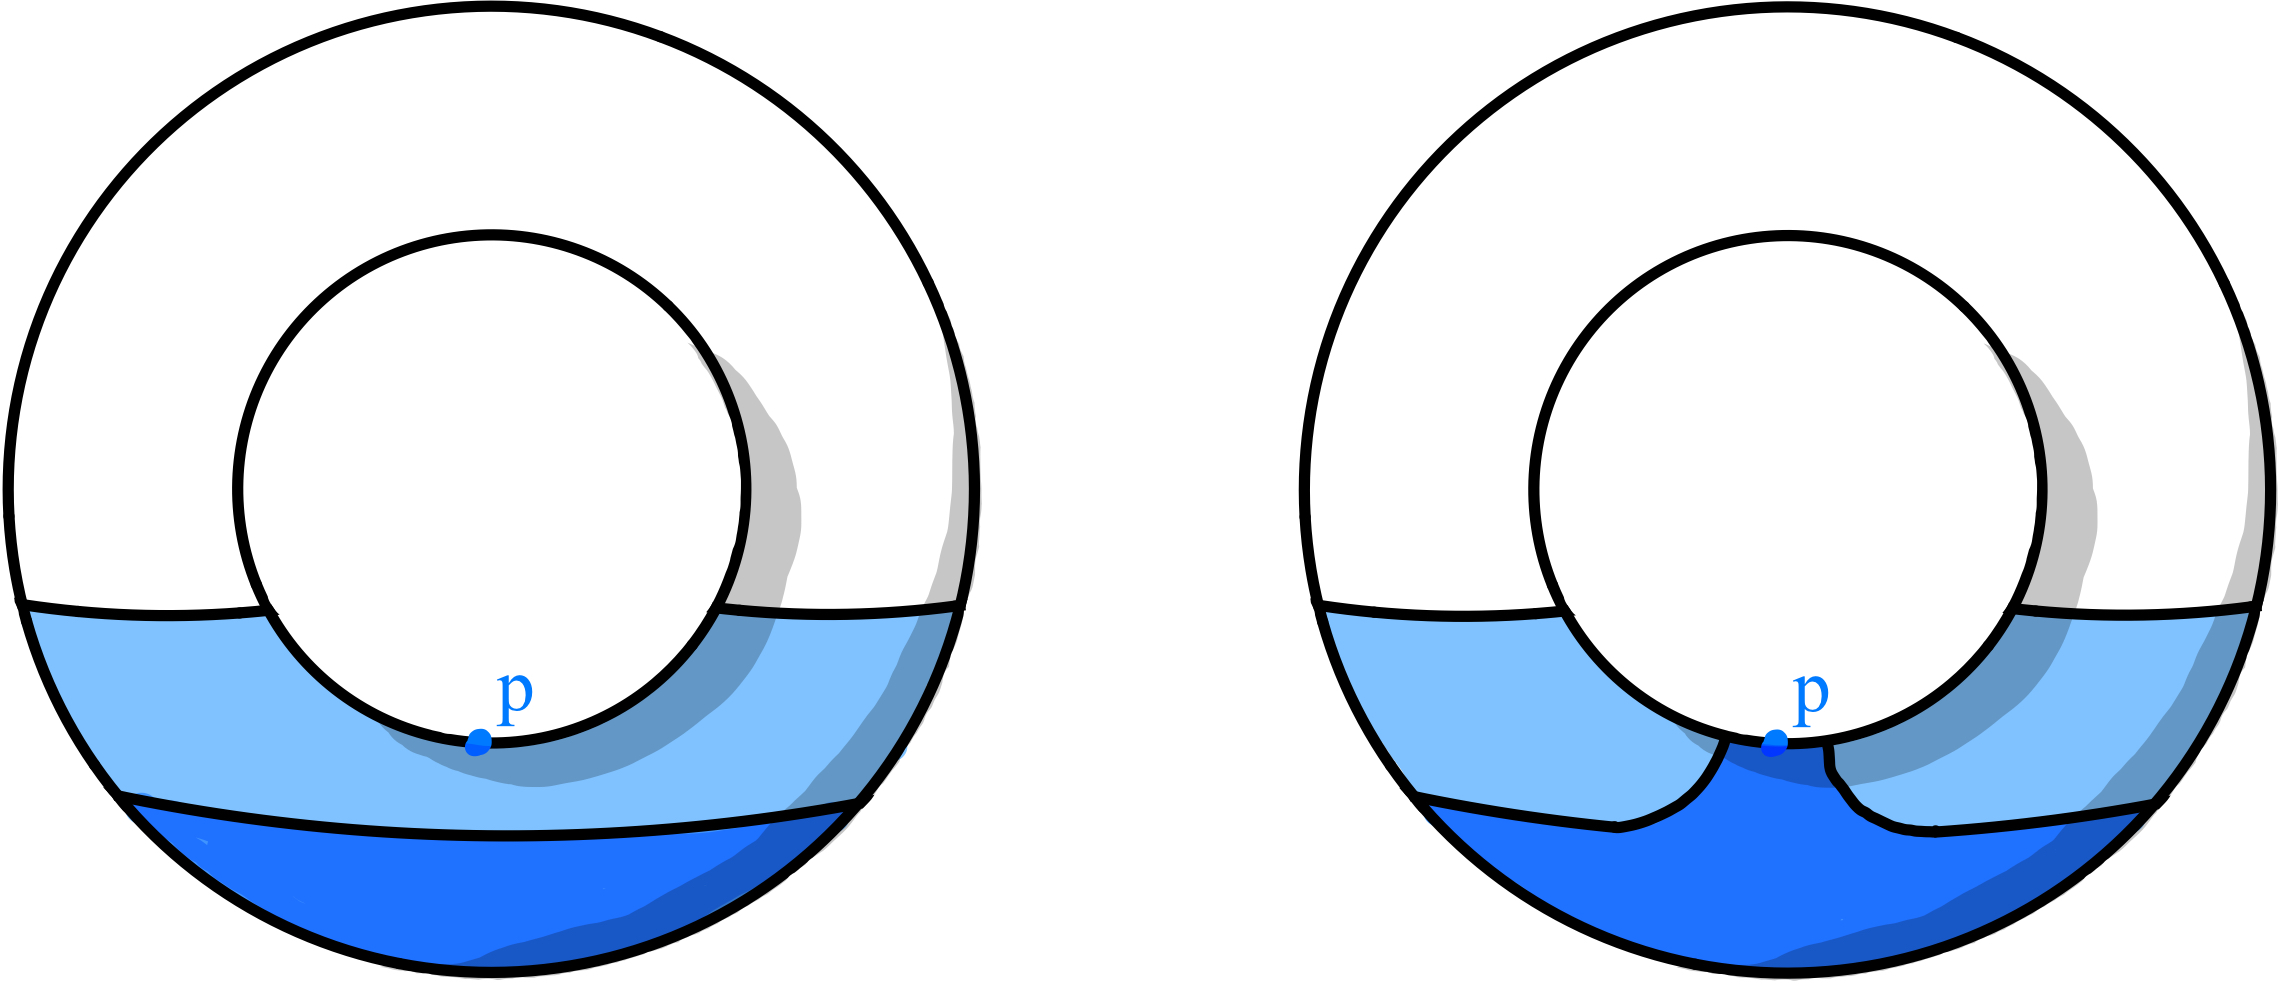
\includegraphics[width=0.8\linewidth]{../resources/Me-Diagram5-sublevelsets-of-f-and-F.jpeg}
        \label{fig:me-diagram5}
        \caption{Die Niveaumengen von $f$ (links) und $F$ (rechts)}
    \end{figure}

    Wir wollen also, dass $M^{c + \varepsilon} = F^{-1}(- \infty, c + \varepsilon]$ 
    gilt und $F^{-1}(-\infty, c - \varepsilon]$ fast dasselbe ist wie 
    $M^{c - \varepsilon}$, nur dass $F^{-1}(-\infty, c - \varepsilon]$ einen "Henkel"
    enthält der den kritischen Punkt $p$ enthält.

    Wir benutzen das Morse-Lemma~\ref{satz: morse-lemma}:
    Wir finden lokale Koordinaten $\phi = (u_1, \dots, u_n)$ in einer Umgebung $U$ von $p$, sodass 
    \[ f = c - u_1 - \dots - u_k + u_{k + 1} + \dots + u_n \]
    und
    \[ u_1 (p) = \dots = u_n(p) = 0 . \]
    Sei $\eps$ ohne Beschränkung der Allgemeinheit klein genug, sodass $f^{-1}[c - \eps, c + \eps]$ 
    kompakt ist und die Kreisscheibe $\{ x \in \R^n : \| x \|^2 \leq 2 \eps \}$ im Bild von $\phi$ 
    enthalten ist. Wähle nun die $k$-Zelle 
    \[ e^k := \{ q \in M : u_1^2 (q) + \dots + u_k^2 (q) \leq \eps \text{ und }
        u_{k + 1} (q) = \dots = u_n (q) = 0 \} . \]
    Wir bekommen folgende Situation:
    \begin{figure}[H]
        \centering
        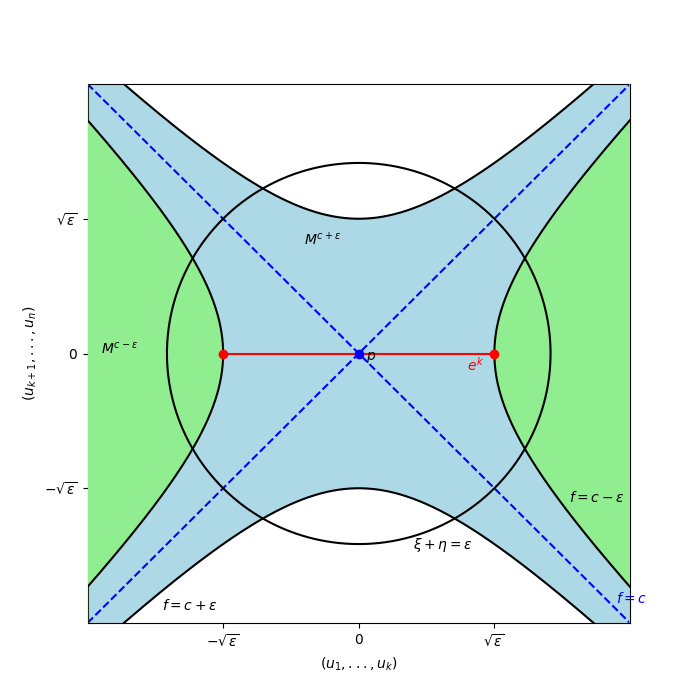
\includegraphics[width=0.5\linewidth]{../resources/Me-Diagram6-U-parameterized.png}
        \label{fig:me-diagram6}
    \end{figure}
    $F$ wird nun so definiert, dass eine Umgebung der $k$-Zelle $e^k$ ein wenig abgesenkt wird.
    Sei $\mu \colon \R \to \R$ eine glatte Funktion mit den Eigenschaften
    \begin{enumerate}
        \item $\mu(0) > \eps$
        \item $\mu (r) = 0$ falls $r \geq 2 \eps$
        \item $-1 < \mu' (r) \leq 0$ für alle $r \in \R$ .
    \end{enumerate}
    Sei dann $F$ außerhalb von $U$ gleich $f$, und innerhalb von $U$ setze
    \[ F = f - \mu ( u_1^2 + \dots + u_k^2 + 2 u_{k + 1}^2 + \dots + 2 u_n^2) . \]
    Man überprüft dann die drei Behauptungen
    \begin{enumerate}
        \item $F^{-1}(- \infty, c + \eps] = M^{c + \eps}$,
        \item $F^{-1}(- \infty, c - \eps]$ ist Deformationsretrakt von $M^{c + \eps}$,
        \item $M^{c - \eps \cup e^k}$ ist Deformationsretrakt von $F^(- \infty, c - \eps]$.
    \end{enumerate}
    Die zweite Behauptung folgt aus dem ersten Deformationslemma.
    
    Den detaillierten Beweis findet man zum Beispiel in \cite{milnor}.
\end{proof}

Mit diesen beiden Aussagen kommt man schon sehr weit. Die berühmten Morse- \\Ungleichungen lassen
sich mit ein bisschen linearer Algebra an exakten Sequenzen leicht daraus folgern. Man kann sogar
zeigen, dass jede Mannigfaltigkeit den Homotopietypen eines CW-Komplexes 
(siehe Def.~\ref{def: cw-komplex}) besitzt, wie es zum Beispiel Milnor tut. Die folgenden Kapitel 
geben eine etwas eleganterere Sicht auf die Thematik, die in gewisser Hinsicht stärkere Aussagen
liefert:

\textit{Kompakte} Mannigfaltigkeiten haben nicht nur den selben Homotopie-Typen eines CW-Komplexes, 
sondern sie sind sogar CW-Komplexe, und wir können uns die zelluläre Homologie, die aus der 
CW-Struktur hervorgeht sogar auf eine einfache Art und Weise erklären.

\chapter{Der Morse-Komplex}
In diesem Kapitel wird der Morse Komplex definiert und gezeigt, dass der 
Morse-Komplex ein Kettenkomplex ist.

\section{Die stabile- und instabile Mannigfaltigkeit und die Smale-Bedingung}

\begin{definition}[Stabile- und instabile Mannigfaltigkeit]
    \label{def: stabile und instabile mannigfaltigkeit}
    Es sei $f \colon M \to \R$ eine Morse-Funktion, $p$ ein kritischer Punkt von $f$ und $X$ ein
    Pseudo-Gradientenfeld von $f$. Die stabile Mannigfaltigkeit von $p$ ist die Menge
    \[ \stab (p) = \left\{ q \in M : \lim_{t \to + \infty} \phi_t(q) = p \right\} \]
    und die instabile Mannigfltigkeit ist
    \[ \unst (p) = \left\{ q \in M : \lim_{t \to - \infty} \phi_t(q) = p \right\} . \]
\end{definition}

Bevor wir die stabile- und instabile Mannigfaltigkeit eines kritischen Punktes weiter untersuchen, 
fixieren wir ein Paar Notationen zu Morse Umgebungen. Für das gesamte Kapitel ist diese Vorstellung
von Morse-Umgebungen wichtig.

\begin{definition}[Notationen zu Morse Umgebungen]
    \label{def: notation morse umgebung}
    Zuerst untersuchen wir eine quadratische Formin $\R^n$, die die Form hat wie Funktionen in Morse
    Umgebungen, also $Q \colon \R^n \to \R$ mit
    \[ Q(x_1, \dots, x_n) = - x_1^2 - \dots - x_k^2 + x_{k + 1}^2 + \dots + x_n^2 \]
    für ein $1 \leq k \leq n$.
    Mit $x_- := (x_1, \dots x_k)$ und $x_+ := (x_{k + 1} \dots x_n)$ gilt dann
    \[ Q = - \| x_- \|^2 + \| x_+ \|^2 . \]
    Der Gradient von $Q$ ist mit dem Standardskalarprodukt auf $\R^n$
    \[ \grad Q (x_-, x_+) = 2(x_-, x_+) . \]
    Es seien $\eps, \eta > 0$. Dann definiere die Menge
    \[ U(\eps, \eta) := \left\{ x \in \R^n : - \eps \leq Q(x) \leq \eps 
    \text{ und } \| x_- \|^2 \| x_+ \|^2 \leq \eta(\eps + \eta) \right\} := U . \]
    Wir definieren außerdem
    \begin{align*}
        \del_{\pm} U := & \left\{ x \in U: Q(x) = \pm \eps \text{ und } \|x_{\mp} \|^2 \leq \eta \right\} 
            \text{ und} \\
        \del_0 U := & \left\{ x \in \del U: \| x_- \|^2 \| x_+ \|^2 = \eta(\eps + \eta) \right\} .
    \end{align*}
    Dann setzt sich der Rand von $U$ aus diesen drei Teilen zusammen, also
    \[ \del U = \del_+ \cup \del_- \cup \del_0 . \]
    $\del_0 U$ ist parallel zu den Trajektorien des negativen Gradienten von $Q$. $\del_+ U$ und 
    $\del_- U$ sind orthogonal zu den Trajektorien des negativen Gradienten von $Q$, wobei die 
    Trajektorien in $\del_+ U$ in die Menge $U$ eintreten und sie in $\del_- U$ wieder verlassen. 
    Wir setzen nun $V_- = \langle e_1, \dots, e_k \rangle$ und 
    $V_+ = \langle e_1, \dots, e_n \rangle \subseteq \R^n$. $V_+$ ist der größte Vektorraum, 
    auf dem $\opd^2 Q (0) (\cdot, \cdot)$ positiv definit ist und $V_-$ der größte Vektorraum, auf dem 
    $\opd^2 Q (0) (\cdot, \cdot) (0)$ negativ definit ist. 
    Es gilt 
    \[ \del U \cap V_{\pm} \subseteq \del_{\pm} U . \]
    $0$ ist der einzige kritische Punkt von $Q$ und ist offensichtlich nicht degeneriert. Damit ist $Q$
    eine Morse Funktion und es gilt 
    $\stab (0) = V_+$ und $\unst (0) = V_-$.

    Ist nun $f \colon M \to \R$ eine Morse Funktion, $p$ ein kritischer Punkt von $f$ und $(V, \psi)$
    eine Morse Umgebung von $p$, dann gilt $f \circ \psi^{-1} = Q + f(p)$. Sind $\eps$ und $\eta$
    klein genug, dann ist $U \subset \psi(V)$. Wir nennen 
    $\Omega (p, \eps, \eta) = \Omega (p) = \psi^{-1}(U)$, und 
    $\del_{\pm} \Omega (p) = \psi^{-1}(\del_{\pm}U)$ und $\del_0 \Omega (p) = \psi^{-1} (\del_0 U)$.
    Dann ist 
    \[ \psi(\stab (p) \cap \Omega (p)) = V^+ \cap U \] 
    und 
    \[ \psi(\unst (p) \cap \Omega (p)) = V^- \cap U . \]
    Wir können uns also mit dieser Notation die stabile- und instabile Mannigfaltigkeit (wenigstens 
    in einer Umgebung von $p$) sehr gut vorstellen.

    \begin{figure}[ht]
        \centering
        \begin{minipage}{.4\textwidth}
          \centering
          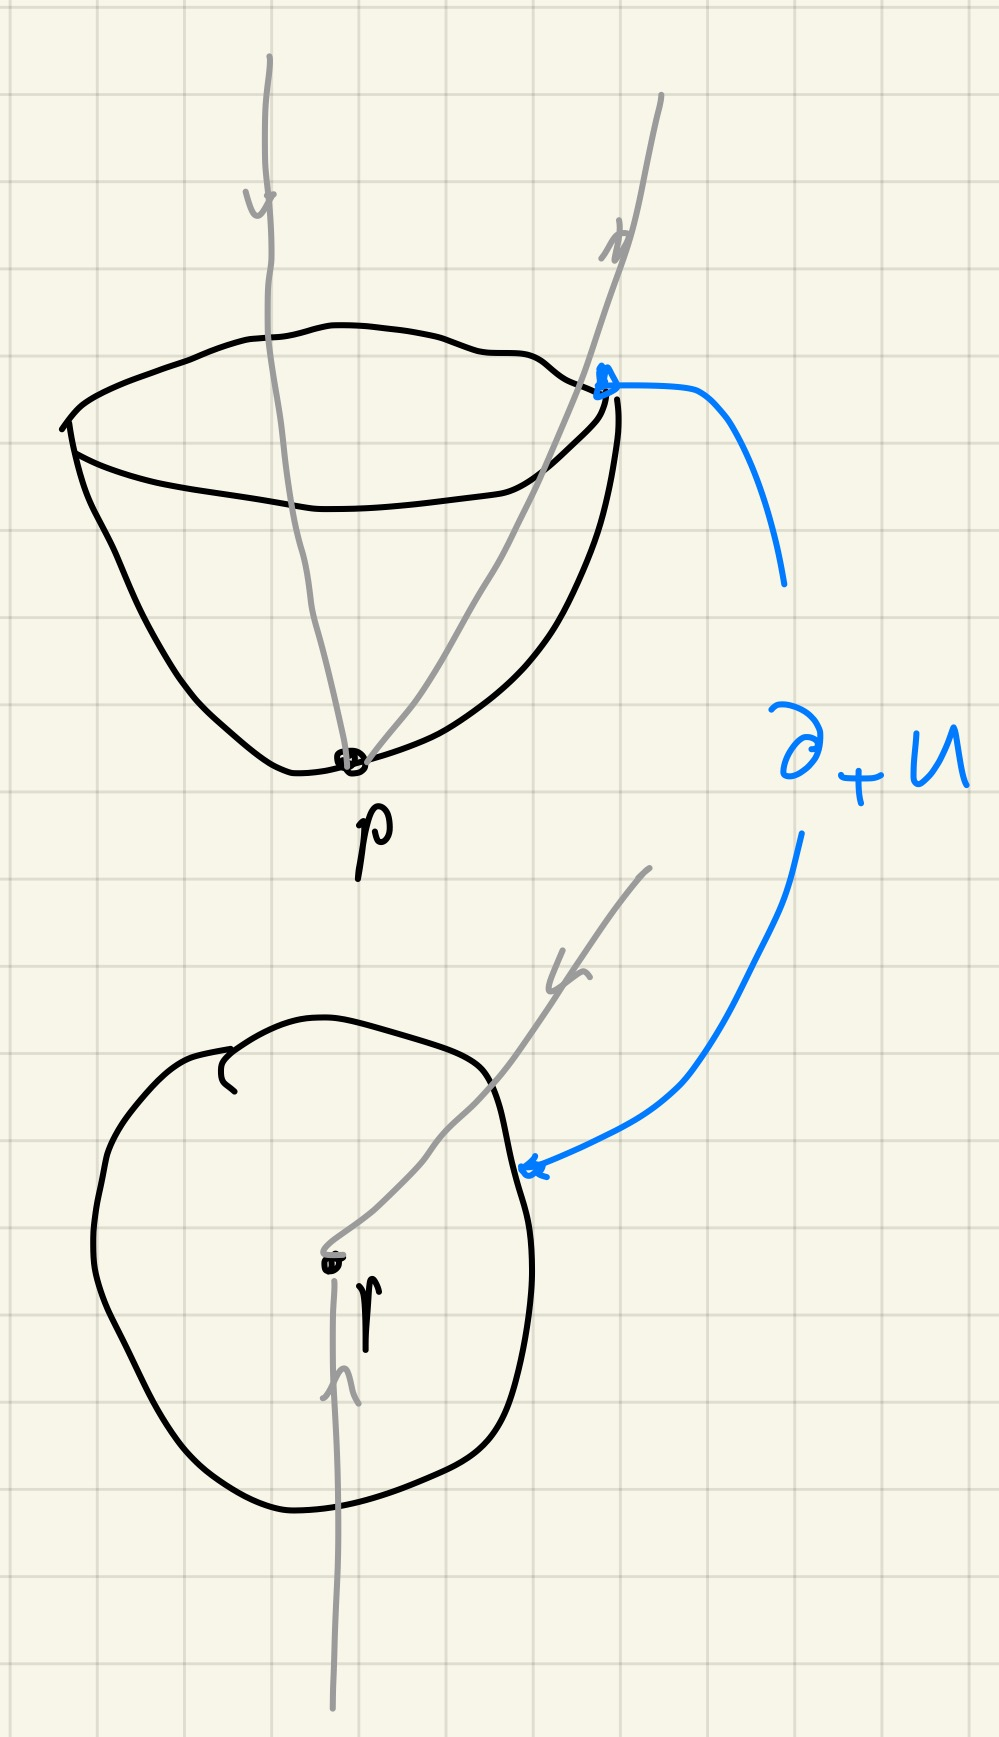
\includegraphics[width=.4\linewidth]{../resources/def-notation-morse-umgebung-1.JPG}
          \captionof{figure}{Index $0$}
          \label{fig: morse umgebung ind 0}
        \end{minipage}%
        \begin{minipage}{.4\textwidth}
          \centering
          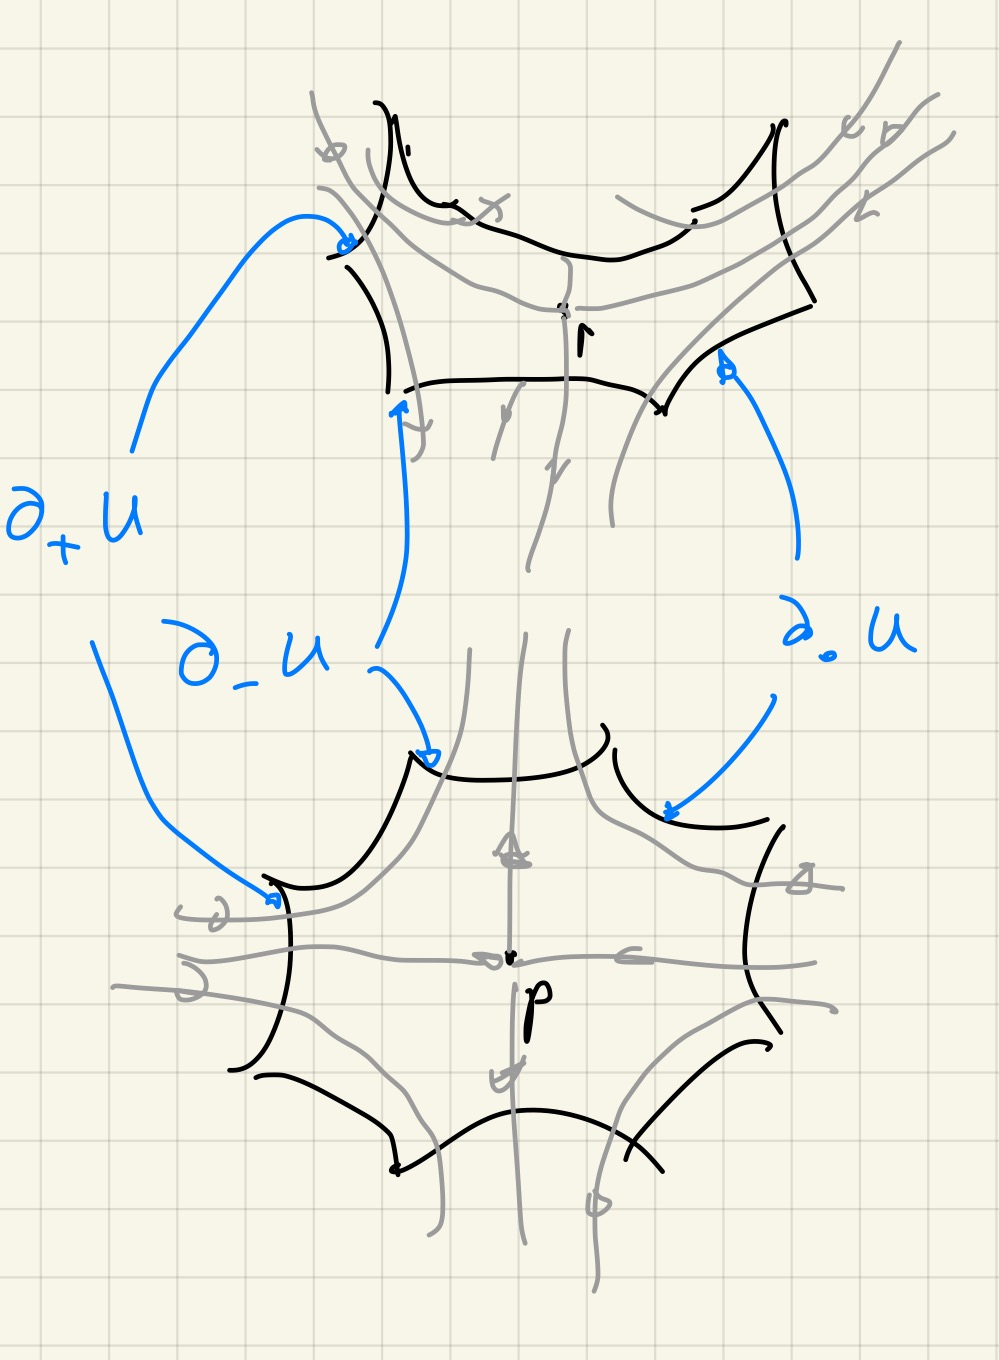
\includegraphics[width=.4\linewidth]{../resources/def-notation-morse-umgebung-2.JPG}
          \captionof{figure}{Index $k$, $0 < k < n$}
          \label{fig: morse umgebung ind k}
        \end{minipage}
    \end{figure}

    $\eps$ und $\eta$ werden häufig in der Notation ausgelassen.
\end{definition}

Mit dieser Vorstellungen von Morse-Funktinoen können wir die folgende Aussage beweisen.

\begin{prop}
    Ist $f \colon M \to \R$ eine Morse Funktion und $p$ ein kritischer Punkt von $f$, dann sind
    $\stab (p)$ und $\unst (p)$ Mannigfaltigkeiten mit 
    \[ \dim \unst (p) = n - \dim \stab (p) = \Index (p) \]
\end{prop}

\begin{proof}
    Es sei $(\psi, V)$ eine Morse Karte um $p$ und $\Omega(p) \subseteq V$ in einer Form wie 
    in ~\ref{def: notation morse umgebung}. Es sei außerdem $\phi$ der Fluss eines 
    Pseudo-Gradientenfeldes von $f$. Dann ist 
    \[ \Phi \colon \del_+ \Omega (p) \cap \stab (p) \times \R \to M ; \; \Phi (q, t) = \phi_t(q) \]
    eine Einbettung und es gilt 
    \[ \stab (p) = \Ima \Phi \cup \psi^{-1}(U \cap V_+) . \]
    Tatsächlich ist 
    \[ \stab (p) - \Ima \Phi = \{ p \} , \]
    denn $\lim_{t \to \infty} \phi_t(q) = p$ für $q \in \del_+ \Omega (p) \cap \stab (p)$. 
    Außerdem ist 
    \[ \del_+ U \cap V_+ = \{ x \in \R^n: \| x_+ \|^2 = \eps \} \diffeo S^{n - k - 1} , \] 
    denn für alle $x \in V_+$ gilt sowieso schon $x_- = 0$. Also ist $\stab(p)$ diffeomorph zum Raum 
    $S^{n - k - 1} \times (-\infty, \infty]/\sim$, in dem alle Punkte in $\infty$ zusammengeklebt 
    werden. Dieser Quotient ist wiederum diffeomorph zur offenen Kreisscheibe mit Dimension $n - k$.
    Genauso zeigt man, dass $\unst (p)$ diffeomorph zur offenen Kreisscheibe mit Dimension $k$ ist.
\end{proof}

\begin{prop}
    \label{prop: trajektorien enden in kritischen punkten}
    Es sei $f \colon M \to \R$ eine Morse-Funktion und $X$ ein Pseudo-\\Gradientenfeld von $f$. 
    Sei außerdem $M$ kompakt. Ist dann $\phi$ der Fluss von $X$, dann existieren für jeden Punkt 
    $p \in M$ kritische Punkte $q$ und $r$ von $f$, sodass
    \[ \lim_{t \to + \infty} \phi_t(p) = q \;\;\; 
    \text{ und } \;\;\; \lim_{t \to -\infty} \phi_t(p) = r \]
\end{prop}

\begin{proof}
    Wir zeigen die erste Aussage. Seien für jeden kritischen Punkt $p$ $(U_p, \psi_p)$ Morse Karten.
    Es ist $\lim_{t \to + \infty} \phi_t(q) = p$, genau dann wenn
    der Fluss $\phi_{\bullet}(q)$ den Punkt $q$ irgendwann in die Umgebung 
    $\del_+ \Omega (p) \cap \stab(p)$ transportiert. Angenommen $\phi_{\bullet}(q)$ transportiert
    $q$ nie zu einem kritischen Punkt. Jedes mal wenn $\phi_{\bullet}(q)$ also ins Innere einer
    Morse-Umgebung $U_q$ gerät, muss diese Umgebung auch wieder verlassen werden. Da 
    $f \circ \phi_{bullet}(q)$ monoton ist, kann nachdem $\phi_{bullet}(q)$ die Morse-Umgebung 
    $\Omega (p)$ verlassen hat, nie wieder zu dieser zurückgekehrt werden.
    Sei also 
    \[ \Omega = \bigcup_{p \in \Crit(f)} \Omega (p) \]
    und $t_0$ der Zeitpunkt an dem $\phi_{\bullet} (q)$ die Umgebung $\Omega$ das letzte mal verlässt.
    Da $M - \Omega$ keine kritischen Punkte von $f$ enthält existiert ein $\eps_0 > 0$, sodass für 
    alle $x \in M - U$ gilt 
    \[ \opd f (x) ((X(x))) \leq - \eps_ . \]
    Wir rechnen also: Für jedes $t \geq t_0$ gilt
    \begin{align*}
        f(\varphi_t(q) - f(\varphi_{t_0}(q))) = & 
            \int_{t_0}^t \derive[f \circ \phi_{\bullet}(q)]{s} (s) \opd s \\
        = & \int_{t_0}^t \opd f (\phi_s(q)) (X(\phi_s(q))) \opd s \\
        \leq & - \eps_0 (t - t_0) . 
    \end{align*}
    Also für $t \to + \infty$ gilt $f(\phi_t(p)) \to - \infty$. Das kann aber nicht sein, denn da 
    $M$ kompakt ist und $\R$ Hausdorff, ist $f$ eigentlich, also ist $\Ima f$ kompakt. 
    \todo{stimmt das?} Also kann $\phi_{\bullet}(p)$ 
    nicht alle $U_q$ verlassen. aber dann ist 
    \[ \lim_{t \to + \infty} \phi_t(q) = p \]
    für einen kritischen Punkt $p$.
    Genauso zeigt man, dass $\lim_{t \to - \infty} \phi_t(p) = r$ für einen kritischen Punkt $r$.
\end{proof}

\begin{definition}[Smale-Bedingung]
    \label{def: smale-bedingung}
    Es sei $M$ eine Mannigfaltigkeit und $U$ und $V$ Untermannigfaltigkeiten von $M$. Wir sagen 
    $U$ und $V$ sind \textit{transversal} und schreiben $U \pitchfork V$, falls für alle Punkte 
    $p \in U \cap V$ gilt 
    \[ T_pU + T_pV = T_pM . \]
    Ein Vektorfeld $X \in \VFs (M)$ heißt \textit{transversal} zur Untermannigfaltigkeit $U$, falls 
    für alle $p$ in $U$ gilt 
    \[ \langle X(p) \rangle + T_pU = T_pM . \]

    Sei nun $f \colon M \to \R$ eine Morse Funktion und $X$ ein Pseudo-Gradientenfeld von $f$. Dann sagen
    wir, dass $X$ die \textit{Smale-Bedingung} erfüllt, falls für alle kritischen Punkte $p$ und $q$ von 
    $f$ gilt 
    \[ \stab (p) \pitchfork \unst (q) . \]
    Ein Paar $(f, X)$ aus einer Morse-Funktion $f$ und einem Pseudo-Gradientenfeld $X$, das die 
    Smale-Bedingung erfüllt, nennt man \textit{Morse-Smale Paar}.
\end{definition}

\begin{prop}
    \label{prop: schnitt von transversalen untermannigfaltigkeiten}
    Sind $U_1$ und $U_2$ Untermannigfaltigkeiten von einer $n$-\\
    dimensionalen Mannigfaltigkeit $M$ mit 
    Dimensionen $d_1$ und $d_2$, sodass 
    \[ U_1 \pitchfork U_2 , \]
    dann ist $U_1 \cap U_2$ eine Untermannigfaltigkeit von $M$ mit Dimension $d_1 + d_2 - n$.
\end{prop}

\begin{proof}
    Es sei $p \in U_1 \cap U_2$. Da $U_1$ und $U_2$ Untermannigfaltigkeiten sind existieren 
    Karten $(\phi_1, V_1)$ und $(\phi_2, V_2)$ von $M$, sodass 
    \[ \phi_1 = (\phi_1', \phi_1'') \colon V_1 \to 
        \Omega_1 \times \Omega_1' \subseteq \R^{d_1} \times \R^{n - d_1} \]
    mit $\phi_1(V_1 \cap U_1) = \Omega_1 \times \{ 0 \}$ und 
    \[ \phi_2 = (\phi_2', \phi_2'')\colon V_2 \to 
        \Omega_2 \times \Omega_2' \subseteq \R^{d_2} \times \R^{n - d_2} \]
    mit $\phi_2(V_2 \cap U_2) = \Omega_2 \times \{ 0 \}$. Definiere 
    \[ \phi'' = (\phi_1'', \phi_2'') \colon 
        M \supseteq V_1 \cap V_2 \to \R^{n - d_1} \times \R^{n - d_2}. \]
    Dann ist 
    $(\phi'')^{-1}(0) = (U_1 \cap V_1) \cap (U_2 \cap V_2) = (U_1 \cap U_2) \cap (V_1 \cap V_2) := V$.
    Wir wollen nun den Satz über reguläre Werte anwenden, aber dafür müssen wir zeigen, dass 
    $\opd \phi'' (p)$ surjektiv ist. Bemerke, dass 
    $\opd \phi'' (p) = \opd (\phi''_1, \phi''_2) (p) = (\opd \phi''_1 (p), \opd \phi''_2 (p))$.
    Es sei $v \in T_p \R^{n - d_1}$ und $w \in T_p\R^{n - d_2}$. Da $\opd \phi''_1 (p)$ und 
    $\opd \phi''_2 (p)$ surjektiv sind, und da $U_1$ und $U_2$ transversal sind, 
    existieren $v_1' + v_2', w_1' + w_2' \in T_pU_1 + T_pU_2$, sodass 
    $\opd \phi''_1 (p) (v_1 + v_2) = \opd \phi''_1 (p) (v_2) = v$ und 
    $\opd \phi''_2 (p) (w_1 + w_2) = \opd \phi''_2 (p) (w_1) = w$.
    Die ersten Gleichheiten gelten, da $T_p U_1$ der Kern von $\opd \phi''_1 (p)$ und 
    $T_p U_2$ der Kern von $\opd \phi''_2 (p)$ sind. Dann gilt
    \[ \opd \phi'' (p) (w_1' + v_2')  = 
        ( \opd \phi''_1 (p) (v_2'), \opd \phi''_2 (p) (w_1')) = (v, w) . \]
    Wir können also den Satz über reguläre Werte anwenden, dann ist $V$ eine Untermannigfaltigkeit
    mit Dimension $n - ((n - d_1) + (n - d_2)) = d_1 + d_2 - n$. Dann ist auch $U_1 \cap U_2$
    eine Untermannigfaltigkeit von Dimension $d_1 + d_2 - n$.
\end{proof}

Dann folgt direkt:

\begin{prop}
    Es sei $f \colon M \to \R$ eine Morse Funktion und $p$ und $q$ kritische Punkte von mit Index $k_1$
    und $k_2$ respektive. Falls $X$ die Smale-Bedingung erfüllt ist
    \[ \mathcal{M} (p, q) := \unst (p) \cap \stab (q) = 
        \left\{ r \in M : \lim_{t \to - \infty} \phi_t(p) \text{ und } 
        \lim_{t \to + \infty} \phi_t(q) \right\} \]
    ist eine Mannigfaltigkeit mit Dimension $k_1 - k_2$.
\end{prop}

Der Raum $\mathcal{M} (p, q)$ beinhaltet alle Punkte, die auf Trajektorien zwischen den kritischen
Punkten $p$ und $q$ liegen. 

\todo{Zeichnung}

\begin{prop}
    \label{prop: wohldefiniertheit von Lt}
    $\R$ wirkt via $(p, t) \mapsto \phi_t(p)$ auf $\mathcal{M}(p, q)$. Sind $p$ und $q$ kritische 
    Punkte mit $p \neq q$ und Indizes $k_1$ und $k_2$, dann ist 
    \[ \Lt (p, q) = \mathcal{M} (p, q) / \R \]
    eine $k_1 - k_2 - 1$-dimensionale Mannigfaltigkeit und es gilt 
    \[ \Lt (p, q) \diffeo \mathcal{M} (p, q) \cap f^{-1}(c) \]
    für einen regulären Wert $c$ zwischen $f(p)$ und f(q)
    (Wir können ohne Beschränkung der Allgemeinheit annehmen, dass $f(p) \neq f(q)$).
\end{prop}

\begin{proof}
    Die Gruppenwirkung ist frei, denn in $\mathcal{M} (p, q)$
    sind keine kritischen Punkte, da $p \neq q$. Es sei $x$ in $\mathcal{M} (p, q)$. 
    Ist nun $t \neq 0$, dann gilt da $f \circ \phi_{\bullet}(x)$ streng monoton ist 
    $f(\phi_t(x)) \neq f(\phi_0(x)) = f(x)$, also $\phi_t(x) \neq x$.

    Es sei nun $c$ ein regulärer Wert zwischen $f(p)$ und $f(q)$. $f^{-1}(c)$ ist eine 
    $n - 1$-dimensionale Mannigfaltigkeit, und für das Pseudo-Gradientenfeld $X$ gilt 
    $X \pitchfork f^{-1}(c)$, und da für jeden Punkt $a$ gilt $X(a) \in T_a \mathcal{M} (p, q)$
    ist $f^{-1}(c) \cap \mathcal{M} (p, q)$ eine $k_1 - k_2 - 1$-dimensionale Mannigfaltigkeit.
    Sei 
    \[ \iota \colon \mathcal{M} (p, q) \cap f^{-1}(c) \to \mathcal{M}(p, q)\] 
    die Inklusion und 
    \[ p \colon \mathcal{M} (p, q) \to \Lt (p, q) \] 
    die Quotientenabbildung. $p \circ \iota$ ist bijektiv und stetig, und ist 
    $U \subseteq \mathcal{M} (p, q)$ offen, dann ist $p \circ \iota (U)$ offen in $\Lb (p, q)$. 
    Also ist $p \circ \iota$ ein Homeomorphismus und $\Lt (p, q)$ ist Hausdorff, also ist $\Lt (p, q)$
    eine Mannigfaltigkeit, und es gilt sogar
    \[ \Lt (p, q) \diffeo \mathcal{M} (p, q) \cap f^{-1}(c) \]
\end{proof}

Der Raum $\Lt (p, q)$ enthält für jede Trajektorie, die zwischen den kritischen Punkten $p$ und $q$ 
verläuft einen Repräsentanten. Später wird $\Lt (p, q)$ benutzt, um den Morse-Komplex zu definieren.
Die Smale Bedingung ist also für unsere Zwecke wichtig.

Wir gewinnen auch eine wichtige Erkenntnis: 

\begin{corollary}
    Der Index von kritischen Punkten verringert sich entlang von Trajektorien. Denn falls 
    $\Index (p) \leq \Index (q)$, dann ist die Dimension von $\Lt (p, q)$
    kleiner $0$, also ist dann $\Lt (p, q) = \varnothing$.
\end{corollary}

Um den Morse Komplex für jede (kompakte) Mannigfaltigkeit definieren zu können, muss noch gezeigt
werden, dass auf jeder Mannigfaltigkeit tatsächlich ein Morse-Smale Paar existiert. 
Sogar noch stärker ist die folgende Aussage:

\begin{theorem}[Satz von Smale-Kupta]
    Es sei $M$ eine Mannigfaltigkeit mit Rand und $f$ eine Morse-Funktion. Es sei $\Omega$ die 
    Vereinigung von Morse-Umgebungen von allen kritischen Punkten. Sei $X$ ein Pseudo-Gradientenfeld 
    von $f$. Dann existiert ein Pseudo-Gradientenfeld $X'$ von $f$, das die Smale Bedingung erfüllt, 
    das innerhalb von $\Omega$ gleich $X$ ist und für das gilt:

    Für jedes $\eps > 0$, jeden Atlas $(\phi_i, U_i)_{i \in I}$ von $M$ und alle $i \in I$ existiert 
    für jede Kompakte Teilmenge $K_i \subseteq U_i$ ein Vektorfeld $X'$, sodass 
    \[ \| \opd \phi_i^{-1} (\cdot) (X') - \opd \phi_i^{-1} (\cdot) (X) \| < \eps . \]
\end{theorem}

\begin{proof}
    Der Satz wurde von S. Smale in \cite{smale1} bewiesen.
\end{proof}
\section{Der Morse-Komplex und der Raum der gebrochenen Trajektorien}

Wir sind nun bereit, den Morse-Komplex mit Koeffizienten in $\F_2$ (wenigstens) hinzuschreiben.
Wir fixieren für den \textbf{gesamten Rest der Arbeit}: 
\begin{itemize}
    \item eine glatte \textbf{kompakte} Mannigfaltigkeit $M$.
    \item ein Morse-Smale Paar $(f, X)$.
\end{itemize}
Die Notation, die wir zu Morse-Umgebungen in~\ref{def: notation morse umgebung} entwickelt haben 
wird weiterhin wichtig sein. Definiere $C_k (M, (f, X))$ als das $\F_2$-Modul, 
das von den kritischen Punkten von $f$ mit Index $k$ erzeugt wird, also
\[ C_k = \left\{ \sum_{p \, \in \, \Crit_k (f)} a_p \cdot p : a_p \in \F_2 \right\} . \] 
Außerdem sei 
$n_X(p, q) = \# \Lt (p, q) \mod 2$. Dann definiere für einen kritischen Punkt $p$ mit Index $k + 1$:
\[ \del_X (p) := \sum_{q \, \in \, \Crit_{k}(f)} n_X(p, q)p . \]

Das Ziel dieses Abschnittes ist es zu zeigen, dass der Komplex $C_{\ast}(M, (f, X))$ wohldefiniert
ist, also dass gilt $n_X (p, q) < \infty$, und dass es ein Kettenkomple ist, also dass 
$\del_X \circ \del_X = 0$. 
% Sobald das gezeigt wurde ist es recht leicht, den Komplex auch über die 
% ganzen Zahlen zu definieren.

\subsection*{Wohldefiniertheit}

\begin{definition}[Der Raum der gebrochenen Trajektorien]
    \label{def: raum der gebrochenen trajektorien}
    Es seien $p$ und $q$ kritische Punkte von $f$. Der \textit{Raum der gebrochenen Trajektorien} ist
    \[ \Lb (p, q) = 
        \bigcup_{k \in \N} \left( \bigcup_{\substack{c_1, \dots, c_{k - 1} \\ \in \Crit(f)}} 
            \Lt (p, c_1) \times \Lt (c_1, c_2) \times \dots 
                \times \Lt (c_{k - 2}, c_{k - 1}) \times \Lt (c_{k - 1}, q) \right) . \]
\end{definition}

Obwohl die Formulierung recht sperrig wirkt ist sie doch intuitiv: 
$\ell \in \Lt (p, q)$ ist eine \glqq Verbindung\grqq{} zwischen den kritischen Punkten $p$ und $q$ 
entlang des Pseudo-Gradientenfeldes $X$. Ein Element 
$(\ell_1, ..., \ell_k) \in \Lt (p, c_1) \times \dots \times \Lt (c_{k - 1}, q) \subseteq \Lb (p, q)$
ist eine \glqq Verbindung\grqq{} zwischen $p$ und $q$ entlang des Pseudo-Gradientenfeldes $X$, die noch 
bei den kritischen Punkten $c_1, \dots, c_{k - 1}$ \glqq Halt\grqq{} macht. 

\begin{figure}[H]
    \centering
    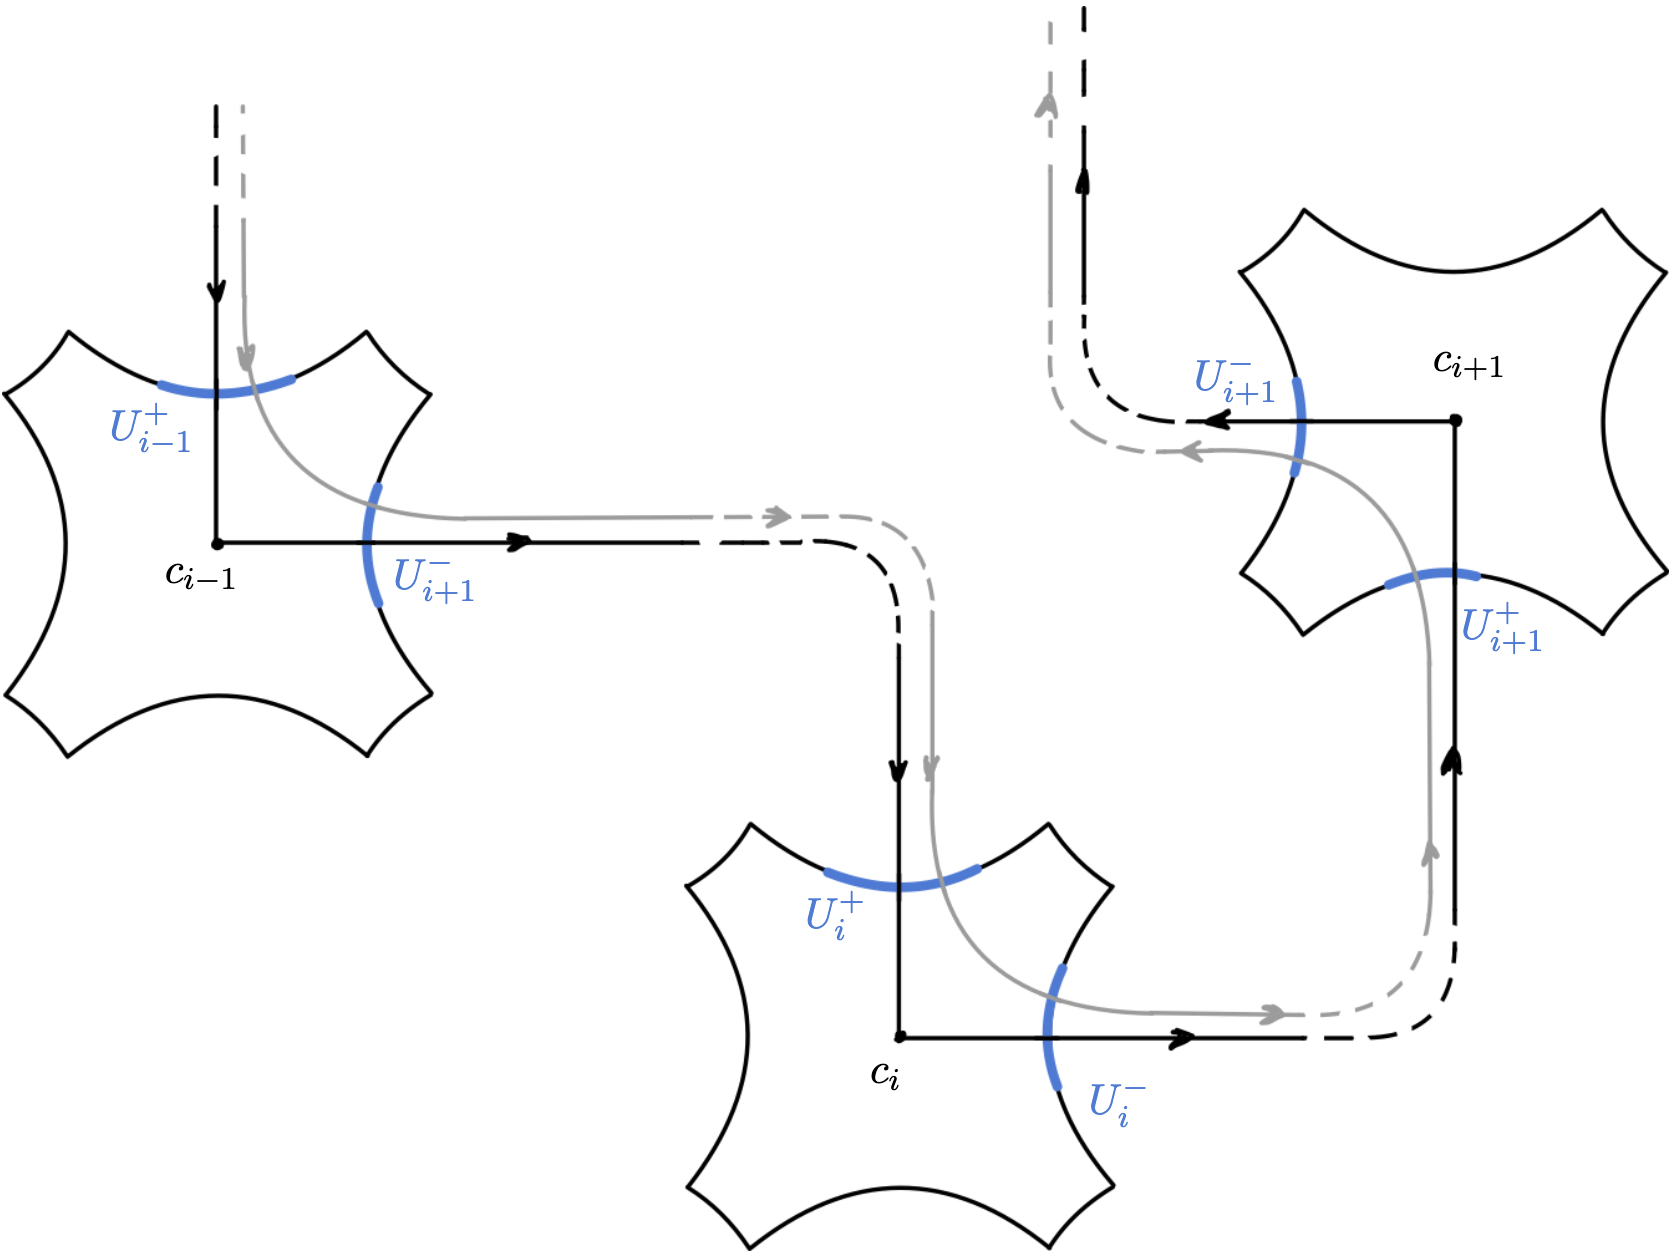
\includegraphics[width=0.5\textwidth]{../resources/broken-trajectories.png}
    \caption{Eine gebrochene Trajektorie (schwarz) und eine nicht gebrochene Trajektorie 
    in einer Umgebung (grau)}
    \label{fig: gebrochene trajektorien}
\end{figure}


Offensichtlich gilt:
\begin{itemize}
    \item Für jedes $\ell \in \Lt (p, c_1) \times \dots \times \Lt (c_{k - 1}, q)$ gilt 
        $\Index (p) < \Index (c_1) < \dots < \Index (c_{k - 1}) < \Index (q)$, denn falls dies nicht
        der Fall ist, ist mindestens einer der Faktoren leer. 
    \item Ist $\Index (p) = \Index (q) + 1$, so ist $\Lb (p, q) = \Lt (p, q)$.
    \item Ist $\Index (p) = \Index (q) + 2$, so ist 
        $\Lb (p, q) = \Lt (p, q) \cup \bigcup_{c \in \Crit (f)} \Lt(p, c) \times \Lt(c, q)$.
\end{itemize}
Tatsächlich sind die beiden letzten Fälle die, die wir am meisten untersuchen werden.
Wir werden sehen, dass man, wie mit der Notation angedeutet, $\Lb (p, q)$ mit einer Topologie 
ausstatten kann, sodass es eine Kompaktifizierung von $\Lt (p, q)$ ist. (In der Tat ist ja 
$\Lt (p, q) \subseteq \Lb (p, q)$).

\begin{definition}[Topologie von $\Lb (p, q)$]
    \label{def: topologie gebrochener trajektorien}
    Wir definieren eine Basis der Topologie von $\Lb (p, q)$. Es seien $p$ und $q$ kritische 
    Punkte von $f$. Wir erinnern uns an unsere Vorstellung von Morse-Umgebungen $\Omega(p)$ wie 
    in~\ref{def: notation morse umgebung}.
    Es sei
    \[ \ell = (\lambda_1, \dots, \lambda_k) 
        \in \Lt (p, c_1) \times \dots \times \Lt(c_{k - 1}, q) \subseteq \Lb (p, q) . \]
    Seien $U_i = \Omega(c_i)$ (nicht unbedingt endgültig gewählte) Morse-Umgebungen von $c_i$ 
    und $U_0$ und $U_k$ Morse-Umgebungen von $p$ und $q$. $\lambda_i \cap \del_+ U_i$ ist der 
    Punkt, an dem $\lambda_i$ in $U_i$ eintritt, und $\lambda_{i + 1} \cap \del_- U_i$ der 
    Punkt, an dem $\lambda_{i + 1}$ die Umgebung $U_i$ verlässt. Es sei $U_i^-$ eine Umgebung von 
    $\lambda_i \cap \del_+ U_i$ in 
    $\del_+ U$ und $U_i^-$ eine Umgebung von $\lambda_{i + 1} \cap \del_- U_i$ in $\del_- U_i$
    (siehe Abb.~\ref{fig: gebrochene trajektorien}). 
    Seien dann $U^- = \bigcup U_i^-$ und $U^+ = \bigcup U_i^+$. Dann definiere ein Element
    $\mathcal{U} (\ell, U^-, U^+)$ aus der Basis wie folgt:

    Wir sagen 
    $\ell' = (\mu_1, ..., \mu_{k'}) \in \Lt (p, c_{i_1}) \times \dots \times \Lt (c_{i_{k'-1}}, q)$
    ist in $\mathcal{U}(\ell, U^-, U^+)$ enthalten, falls $\mu_j \cap U_j^+ \neq \varnothing$
    und $\mu_j \cap U_{j + 1}^- \neq \varnothing$. 

    Eine Menge $\mathcal{V} \subseteq \Lb (p, q)$ heißt dann \textit{offen}, falls $\mathcal{V}$
    die Vereinigung von Elementen aus der Basis ist.
\end{definition}

\begin{remark}
    Die Topologie von $\Lt(p, q)$ als Quotient stimmt mit der von $\Lb(p, q)$ überein.
    Dies ist wieder ersichtlich, wenn wir uns $\Lt (p, q)$ als Schnitt 
    $\mathcal{M} (p, q) \cap f^{-1}(c)$ vorstellen; Die $U^-$ beziehungsweise $U^+$ sind nur 
    offene Umgebungen in den Niveaumengen.
\end{remark}

\begin{prop}
    \label{prop: Lb ist kompakt}
    Es seien $p$ und $q$ kritische Punkte von $f$. Dann ist $\Lb (p, q)$ kompakt.
\end{prop}

Um diese Proposition zu beweisen benötigen wir noch ein Lemma:

\begin{lemma}
    \label{lemma: konvergenz einer folge}
    Es sei $x \in M$ \emph{kein} kritischer Punkt von $f$. Sei außerdem $(x_n)_n$ eine Folge in
    $M$ die gegen $x$ kovnvergiert und seien $y_n$ und $y$ Punkte, die auf den selben Trajektorien
    wie $x_n$ und $x$ liegen. Es gelte außerdem $f(y_n) = f(y)$ für alle $n \in \N$. Dann gilt
    \[ \lim_{n \to + \infty} y_n = y . \]
\end{lemma}

\begin{proof}
    Der Beweis orientiert sich an dem des ersten Deformationslemmas~\ref{satz: erstes deformationslemma}
    (Siehe \cite{audin})
\end{proof}

\begin{proof}[Beweis von Proposition~\ref{prop: Lb ist kompakt}]
    Es sei $(\ell_n)_n$ eine Folge in $\Lb (p, q)$. Um zu zeigen, dass $\Lb (p, q)$ kompakt ist
    müssen wir zeigen, dass $(\ell_n)_n$ eine konvergente Teilfolge besitzt.

    Wir nehmen zuerst an, dass $(\ell_n)_n$ eine Folge in $\Lb (p, q)$ ist.
    Es sei $\ell_n^- \in M$ der Punkt, an dem $\ell_n$ die Morse Umgebung $\Omega(p)$ verlässt 
    und $\ell_n^- \in M$ der Punkt, an dem $\ell_n$ in die Morse Umgebung $\Omega(q)$ eintritt.
    $\ell_n^-$ und $\ell_n^+$ sind im Schnitt von $\del \Omega (p)$ bzw. $\del \Omega (q)$ und 
    der stabilen bzw. instabilen Mannigfaltigkeit. Diese Schnitte sind Kugeloberflächen, also 
    kompakt. Die Folgen $(l_n^-)_n$ und $(\ell_n^+)_n$ haben also konvergente Teilfolgen, wir können 
    demnach ohne Beschränkung der Allgemeinheit annehmen, dass sie konvergent sind. Setze
    \[ \lim_{n \to \infty} \ell_n^- = p^- \text{ und } \lim_{n \to \infty} \ell_n^+ = q^+ . \]
    Sei $\phi$ die von $X$ erzeugte 1-Parameter Gruppe aus Diffeomorphismen, dann ist 
    $\gamma = \phi_{\bullet}(p^-)$ die Trajektorie von $p^-$. Sei 
    $c = \lim_{t \to \infty} \phi_t(p^-)$. Der Punkt $c$ ist nach 
    Proposition~\ref{prop: trajektorien enden in kritischen punkten} ein kritischer Punkt,
    also ist $\gamma \in \Lt (p, c)$.  Es sei $d^+$ der Punkt, an dem $\gamma$ in $\Omega (c)$ 
    eintritt. Da $\phi$ glatt ist, muss wegen der gewählten Topologie 
    aus~\ref{def: topologie gebrochener trajektorien} für $n$ groß genug auch $\ell_n$ die 
    Morse-Umgebung $\Omega (c)$ kreuzen. Sei $d_n^+ \in M$ der Punkt, an dem $\ell_n$ in 
    $\Omega (c)$ eintritt. 
    Dann gilt $d_n^+, d^+ \in \del_+ W$, also gilt $f(d_n^+) = f(d^+)$ für alle $n$. Da $d_n^+$ auf 
    der selben Trajektorie wie $\ell_n^-$ liegt, und $d^+$ auf der selben wie $p^-$,folgt da 
    $\lim \ell_n^- = p^-$ mit dem letzten Lemma~\ref{lemma: konvergenz einer folge}: 
    \[ \lim_{n \to \infty} d_n^+ = d^+ . \]
    Falls $c = q$, dann ist $\lim \ell_n = \gamma \in \Lt (p, q) \subseteq \Lb (p, q)$, also hat 
    dann die Folge $(\ell_n)_n$ eine konvergente Teilfolge. Es sei also $c \neq q$. Dann muss 
    $\ell_n$ die Morse Umgebung $\Omega (c)$ wieder durch einen Punkt $d_n^-$ verlassen. Wie oben 
    können wir ohne Beschränkung der Allgemeinheit annehmen, dass die Folge $(d_n^-)_n$ konvergent 
    ist, da sie zumindest eine konvergente Teilfolge besitzt. Wir definieren dann $d^- := \lim d_n^-$. 
    $d^-$ liegt in der instabielen Mannigfaltigkeit von $c$, denn wäre dies nicht der Fall, dann 
    führt das zu einem Widerspruch:
    
    Angenommen $d^- \notin \unst (c)$. Dann wäre $d^-$ auf der Trajektorie von einem Punkt
    $d^+_{\ast} \in \del_+ \Omega (c)$, der nicht in $\unst (c)$ enthalten ist. Wieder wegen des 
    vorherigen Lemmas~\ref{lemma: konvergenz einer folge} ist dann $\lim d_n^+ = d^+_{\ast}$, also 
    gilt dann $d^+ = d^+_{\ast}$, aber es gilt $d^+ \in \unst (c)$.
    
    Wir können nun wieder mit dem selben Argument zeigen, dass dann die Trajektorie von $d^-$ im
    kritischen Punkt $q$ endet, also liegt dann $\lim \ell_n$ in $\Lt (p, c) \times \Lt (c, q)$.
    \todo{können wir das wirklich?}

    Wir müssen noch zeigen, dass eine Folge $(\ell_n)_n$ in $\Lb (p, q)$ eine konvergente 
    Teilfolge hat. Wegen der Glattheit von $\phi$ können wir annehmen, dass für $n$ groß 
    genug alle $\ell_n$ die Form 
    \[ \ell_n = (\ell^1_n, \dots, \ell^k_n) \in \Lt (p, c_1) \times \dots \times \Lt (c_{k - 1}, q) \]
    haben. Wir finden mit der vorheringen Überlegung komponentenweise eine Teilfolge, sodass wir 
    für den Grenzwert maximal noch $k - 1$ kritische Punkte als \glqq Zwischenstopp\grqq{} einfügen
    müssen. 
\end{proof}

\begin{remark}
    Sind nun $p$ und $q$ kritische Punkte von $f$ mit $\Index (p) = \Index (q) + 1$, dann ist 
    $\Lt(p, q)$ $0$-dimensionale Mannigfaltigkeit. Außerdem ist $\Lt (p, q)$ eine Abgeschlossene
    Teilmenge von $\Lb (p, q)$, und wie wir in der letzten Proposition~\ref{prop: Lb ist kompakt}
    gezeigt haben, ist $\Lb(p, q)$ kompakt, also ist auch $\Lt(p, q)$, und somit endlich.
    Damit ist schon mal $n_X (p, q)< \infty$, also $C_k(M (f, X))$ wohldefiniert.
\end{remark}

\subsection*{Der Morse Komplex ist ein Kettenkomplex}

Wir wollen zeigen, dass der Morse-Komplex tatsächlich ein Kettenkomplex ist, also dass 
$\del_X \circ \del_X = 0$.
Wir rechnen:
\begin{align*}
    \del_X (\del_X (p)) = & \del_X (\sum_{c \in \Crit_k (f)} n_X (p, c) \cdot c) \\
    = & \sum_{q \in \Crit_{k - 1}(f)} \left( 
        \sum_{c \in \Crit_k (f)} n_X(p, c) \cdot n_X(c, q) \right) \cdot q
\end{align*}
und 
\[ \sum_{c \in \Crit_k (f)} n_X(p, c) \cdot n_X(c, q) = 
\# \left( \bigcup_{c \in \Crit_k (f)} \Lt (p, c) \times \Lt (c, q) \right) \mod 2 . \]
Es genügt also zu zeigen, dass für kritische Punkte $p$ und $q$ mit Index $k + 1$ und $k - 1$
gilt, dass $\# \left( \bigcup_{c \in \Crit_k (f)} \Lt (p, c) \times \Lt (c, q) \right)$ gerade ist.

Wir benutzen die folgende Aussage, ohne sie zu beweisen:

\begin{theorem}[Klassifizierung kompakter 1-Mannigfaltigkeiten]
    \label{satz: klassifizierung kompakter 1-mannigfaltigkeiten}
    Es sei $M$ eine kompakte zusammenhängende Mannigfaltigkeit mit Rand. Dann ist
    \begin{itemize}
        \item $M$ diffeomorph zu $S^1$, falls $\del M = \varnothing$
        \item $M$ diffeomorph zu $[0, 1]$, falls $\del M \neq \varnothing$
    \end{itemize}
\end{theorem}

\begin{proof}
    Man kann diese Tatsache mithilfe von Morse-Theorie beweisen, wie es Audain und Damian in 
    \cite{audin} tun, aber ein einfacherer Beweis ist bei Milnor in \cite{milnor2} zu finden.
\end{proof}

\begin{theorem}
    \label{satz: gebrochene trajektorien sind 1-dim mannigfaltigkeit}
    Es seien $p$ und $q$ kritische Punkte von $f$ mit $\Index (p) = k + 1$ und $\Index (q) = k - 1$
    für ein $k \in \N_0$. Dann ist $\Lb (p, q)$ eine 1-dimensionale Mannigfaltigkeit mit Rand, und das
    Innere von $\Lb (p, q)$ ist $\Lt (p, q)$.
\end{theorem}

Mit dieser Proposition folgt dann mit der Kalssifizierung von $1$-Mannigfaltigkeiten mit 
Rand~\ref{satz: klassifizierung kompakter 1-mannigfaltigkeiten} schon, dass der Morse Komplex ein
Kettenkomplex ist, denn dann ist 
\[ \# \left( \bigcup_{c \in \Crit (f)} \Lt (p, c) \times \Lt (c, q) \right) = \del \Lb (p, q) \]
gerade.

\begin{bigproof}
    Wir wissen schon, dass $\Lt (p, q) \subseteq \Lb(p, q)$ eine $1$-dimensionale Mannigfaltigkeit ist. 
    Um sagen zu können, dass $\Lb (p, q)$ eine $1$-dimensionale Mannigfaltigkeit mit Rand ist, und 
    insbsondere, dass $\Lt (p, q)$ das Innere von $\Lb(p, q)$ ist, reicht die folgende Aussage über 
    $\Lb(p, q)$:
    Es sei $c$ ein weiterer kritischer Punkt mit Index $k$.
    Sei $\lambda_1 \in \Lt (p, c)$ und $\lambda_2 \in \Lt (c, q)$. Dann existiert eine offene Umgebung
    $U \subseteq \Lb (p, q)$ von $(\lambda_1, \lambda_2)$, ein $\delta > 0$ und eine (topologische)
    Einbettung $\psi \colon [0, \delta) \to U$, sodass gelten: 
    \begin{enumerate}
        \item $\psi|_{(0, \delta)}$ ist glatt eine glatte Einbettung.
        \item $\psi(0) = (\lambda_1, \lambda_2)$.
        \item $\psi((0, \delta)) \subseteq \Lt (p, q)$.
        \item Für jede Folge $(\ell_n)_n$ in $\Lt (p, q)$ die gegen $(\lambda_1, \lambda_2)$ konvergiert 
            gilt $\ell_n \in \Ima \psi$ für $n$ groß genug.
    \end{enumerate} 
    Die letzte Bedingung stellt sicher, dass sich in $(\lambda_1, \lambda_2)$ keine 
    \say{Kreuzung} befindet (wie zum Beispiel der Klebepunkt bei $S^1 \vee S^1$).
    Wir begeben uns also auf die (recht lange) Suche nach einer solchen Abbildung $\psi$. 

    Wir machen ein Paar Konstruktionen. Sei $\alpha := f(c)$ und $(V, \kappa)$ eine Morse Karte von
    $c$, $\Omega(c)$ wie in der Notation zu Morse Umgebungen~\ref{def: notation morse umgebung}. 
    Dann sind $f(\del_+ \Omega (c)) = \alpha + \eps$ und $f(\del_- \Omega (c)) = \alpha - \eps$ für ein 
    $\eps > 0$. Außerdem setze
    \begin{align*}
        S_+ (c) := & \stab (c) \cap f^{-1}(\alpha + \eps) \diffeo S^{n - k - 1} \\
        S_- (c) := & \unst (c) \cap f^{-1}(\alpha - \eps) \diffeo S^{k - 1} .
    \end{align*}
    Dass $S_+ (c)$ und $S_- (c)$ diffeomorph zu Sphären sind hatten wir schon vorher gesehen.
    Es sei $a_1 \in M$ der Punkt, an dem $\lambda_1$ auf $\Omega(c)$ trifft, also 
    $a_1 = S_+ (c) \cap \lambda_1$, und $a_2$ der Punkt, an dem $\lambda_2$ die Umgebung $\Omega (c)$ 
    wieder verlässt, also $a_2 = S_- (c) \cap \lambda_2$. $\alpha + \eps$ ist kein kritischer Wert 
    von $f$ und es gilt $f^{-1}(\alpha + \eps) \pitchfork \unst (p)$, also ist mit 
    Proposition~\ref{prop: schnitt von transversalen untermannigfaltigkeiten} 
    $P = f^{-1}(\alpha + \eps) \cap \unst (p)$ eine Mannigfaltigkeit mit Dimension 
    $(n - 1) + (k + 1) - n = k$. Da $X$ die Smale-Eigenschaft erfüllt, $P \subseteq \unst (p)$,
    $S_+ \subseteq \stab(c)$, $P, S_+(c) \subseteq f^{-1}(c + \eps)$ und 
    $\dim P + \dim S_+(c) = n - 1$, gilt $P \pitchfork S_+ (c)$. Also ist $P \cap S_+ (c)$
    mit Proposition~\ref{prop: schnitt von transversalen untermannigfaltigkeiten} eine 
    Untermannigfaltigkeit der Dimenion $k + (n - k - 1) - (n - 1) = 0$. Offensichtlich gilt 
    $a_1 \in P \cap S_+ (c)$. Es sei $B^k_{\delta} = \{ x \in \R^k : \| x \| < \delta \}$. Dann 
    existiert eine Umgebung $B$ von $a_1$ in $P$ und ein Diffeomorphismus 
    $\Psi : B \longto B^k_{\delta}$ mit $\Psi(a_1) = 0$, sodass $B \cap S_+ (c) = a_1$ 
    und $B \subseteq \del_+ \Omega (c)$. Wir versuchen die Kernidee des Beweises zu verstehen:

    \begin{figure}
        \centering
        \begin{tikzpicture}
            % Include the image in a node
            \node [
                above right,
                inner sep=0] (image) at (0,0) {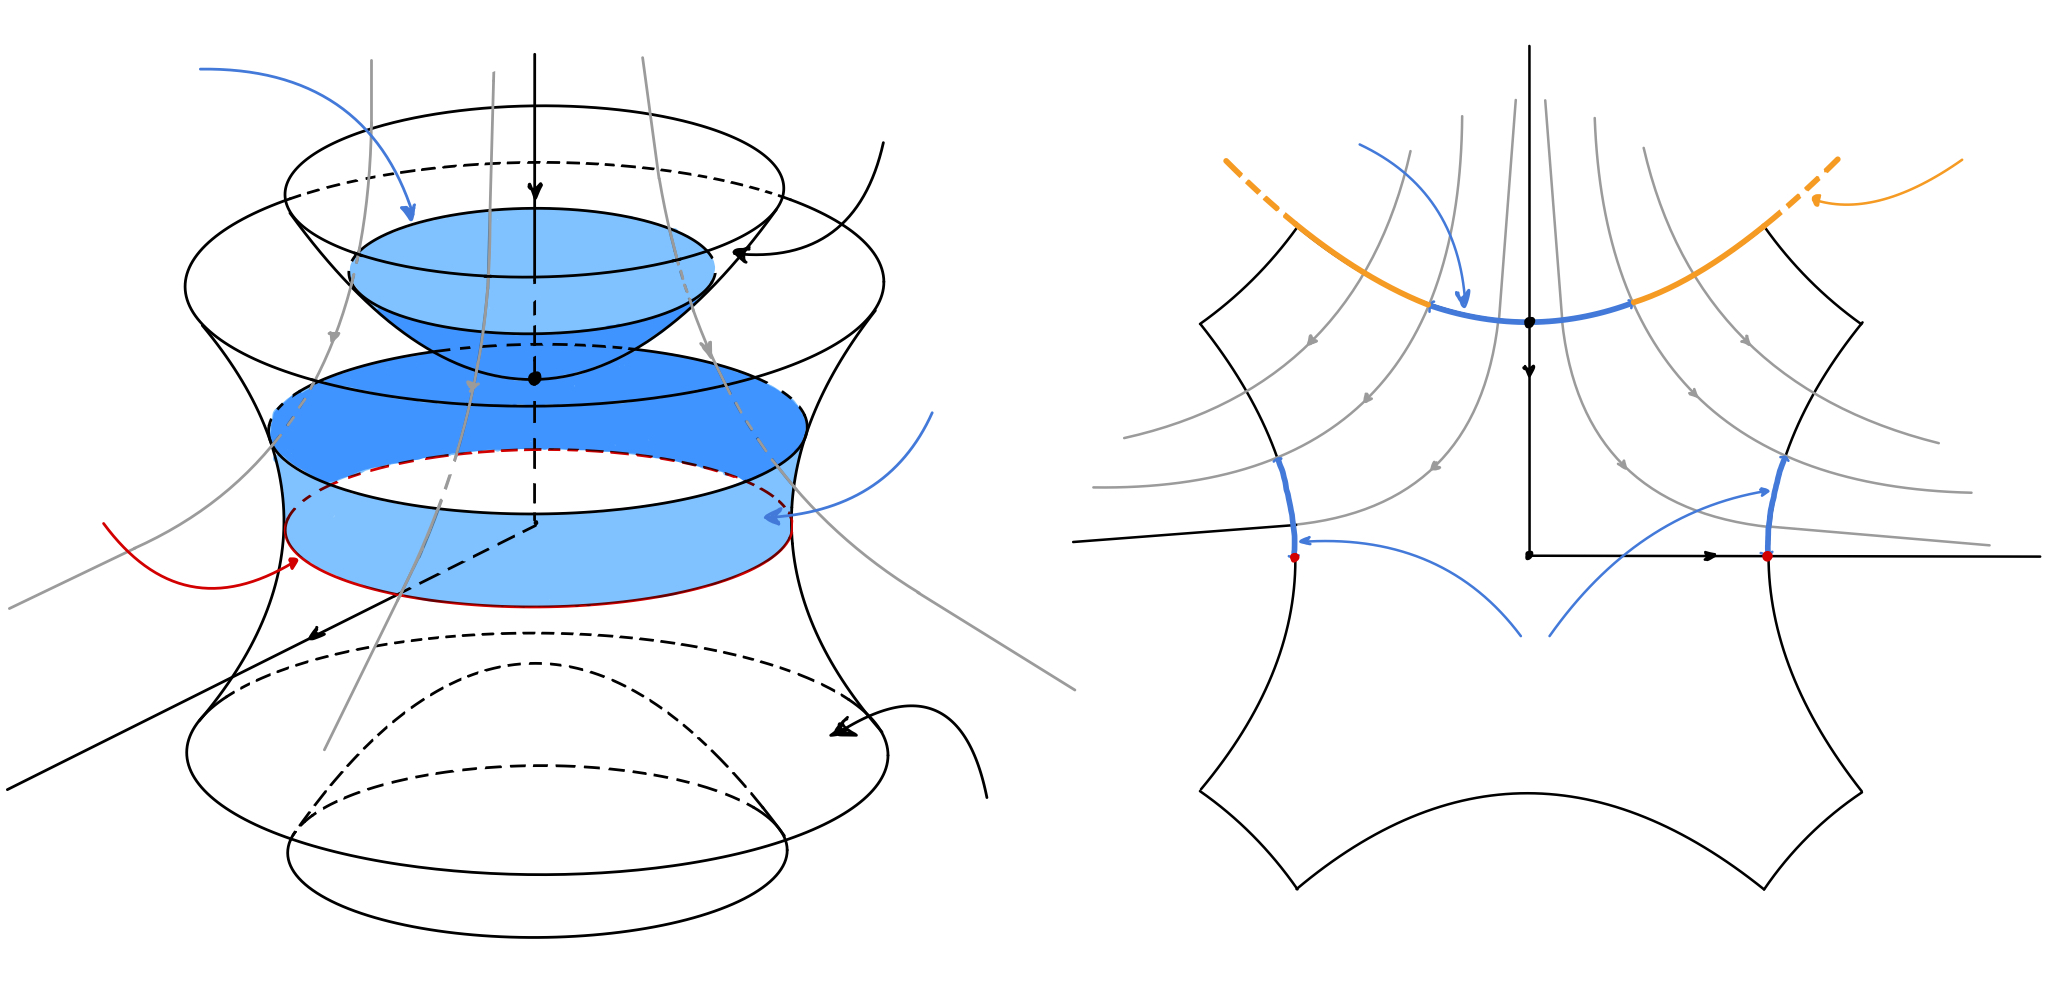
\includegraphics[width=\textwidth]{../resources/lb-ist-1-dim-mfkt.jpeg}};
                
            % Create scope with normalized axes
            \begin{scope}[
            x={($0.02*(image.south east)$)},
            y={($0.05*(image.north west)$)}]
            
            % Annotate left figure
            \node at (13.2, 9.1) {\tiny $c$};
            \node at (13.2, 12.1) {\tiny $a$};

            \node at (13.5, 18.7) {\tiny $\lambda_1$};
            \node at (3.2, 4.8) {\tiny $\lambda_2$};
            
            \node[text=red] at (2.5, 10.1) {\tiny $S_- (c)$};

            \node[text=LightBlue] at (4, 18.5) {\tiny $B$};
            \node[text=LightBlue] at (22.5, 12.3) {\tiny $\Ima (\Phi)$};
        
            \node at (21.5, 17.8) {\tiny $f^{-1}(\alpha + \eps)$};
            \node at (23.8, 3.6) {\tiny $f^{-1}(\alpha - \eps)$};
            
            % Annotate right figure
            \node at (36.6, 8.6) {\tiny $c$};
            \node at (36.5, 13.2) {\tiny $a$};

            \node at (37.6, 18.5) {\tiny $\lambda_1$};
            \node at (48.5, 8.4) {\tiny $\lambda_2$};

            \node[text=red] at (32.4, 8.2) {\tiny $S_-(c)$};
            
            \node[text=LightBlue] at (32.4, 17.4) {\tiny $D$};
            \node[text=LightBlue] at (37, 6.8) {\tiny $\Ima (\Phi)$};

            \node[text=orange] at (47.8, 17.2) {\tiny $P$};
            
            % \draw[lightgray,step=1] (image.south west) grid (image.north east);
            \end{scope}
        \end{tikzpicture}
        \caption{Anschauung von $\Phi$, falls $\Index (c) = 1$ und $M$ $3$-dimensional 
        (links) und $2$-dimensional (rechts)}
        \label{fig: anschauung von phi}
    \end{figure}

    Man betrachte die Abbildungen~\ref{fig: anschauung von phi}.

    Wir versuchen, die Menge $B - a_1$ entlang der Trajektorien von $X$ auf $\del_- \Omega(c)$ via einer 
    Abbildung $\Phi$ einzubetten. Wir werden sehen, dass $Q = \Ima (\Phi) \cup S_+(c)$ eine 
    Mannigfaltigkeit mit Rand ist, und dass dann $Q \cap \stab (q)$ eine $1$-dimensionale
    Mannigfaltigkeit mit Rand ist, und $a_2 \in \del (Q \cap \unst (q))$. Wie 
    in~\ref{prop: wohldefiniertheit von Lt} ist $Q \cap \stab (q) - a_2$ eine Teilmenge von 
    $\Lt (p, q)$, und $a_2 \in \Lt (c, q)$, wenn wir also $a_2 \in \lambda_2$ mit 
    $(\lambda_1, \lambda_2)$ identifizieren, dann bekommen wir unsere Parametrisierung 
    $\psi$ von $\Lb (p, q)$. 
    Also:

    \begin{claim}
        Es sei $\phi$ die von $X$ erzeugte 1-Parameter Gruppe aus Diffeomorphismen. Für jedes 
        $x \in B - a_1$ existiert ein $t_x \in \R$, sodass $\phi_{t_x} (x) \in \del_- \Omega (c)$
        und $x \mapsto t_x$ glatt ist.
    \end{claim}

    \begin{smallproof}
        Via unserer anfangs gewählten Morse Karte $(V, \kappa)$, und da wir ohne Einschränkungen $B$ 
        klein genug wählen können, sodass $B \subseteq \Omega (c)$, können wir annehmen, dass sich 
        alles im $\R^n$ abspielt ; Sei also ohne Beschränkung der Allgemeinheit 
        $f(x_-, x_+) = - \|x_-\| + \|x_+\|$. Dann ist $\phi$ gegeben durch 
        \[ \phi_t(x_-, x_+) = (e^{2t}x_-, e^{-2t}x_+) . \]
        Falls $(x_-, x_+) \in \del_+ U$ und $x_- \neq 0$, dann gilt auch $x_+ \neq 0$. Setze
        \[ t_{(x_-, x_+)} = \frac{1}{2} \ln \left( \frac{\| x_+ \|}{\| x_- \|} \right) . \]
        Dann gilt
        \[ \phi_{t_{(x_-, x_+)}} (x_-, x_+) = 
            \left( \frac{\| x_+ \|}{\| x_- \|} x_-, \frac{\| x_- \|}{\| x_+ \|} x_+ \right) . \]
        Die Zuordnung $(x_-, x_+) \mapsto t_{(x_-, x_+)}$ ist glatt und 
        \begin{align*}
            f(\phi_{t_{(x_-, x_+)}})(x_-, x_+) = & - \| \frac{\| x_+ \|}{\| x_- \|} x_- \|
                +  \| \frac{\| x_- \|}{\| x_+ \|} x_+ \| \\
                = & - \| x_+ \| + \| x_- \| \\
                = & - \eps .
        \end{align*}
        Es folgt $\phi_{t_{(x_-, x_+)}} (x) \in \del_- U$.
    \end{smallproof}

    Wir haben nun also eine Einbettung $\Phi$ von $B - a_1$ entlang der Trajektorien von $X$ gefunden.
    Wie am Anfang besprochen wollen wir jetzt zeigen:

    \begin{claim}
        Ist $\delta$ klein genug, dann ist $Q = \Ima (\Phi) \cup S_+ (c)$ eine $k$ dimensionale 
        Mannigfaltigkeit mit Rand, und es gilt $\del Q = S_- (c)$.
    \end{claim}

    \begin{smallproof}
        Wieder spielt sich alles via $\kappa$ im $\R^n$ ab. Sei wie 
        in~\ref{def: notation morse umgebung} $U = \kappa^{-1}(\Omega (c))$.
        Man betrachte die Projektion
        \[ \pi \colon \R^k \times \R^{n - k} ; \pi (x_-, x_+) = x_- . \]
        und ihre Einschränkung $\del_+ U \to B_{\eta}^k$.
        \todo{weiß net ob das stimmt, naja} Da $S_+ := \kappa(S_+(c)) = (\pi|_{\del_+U})^{-1}(0)$
        und $B \pitchfork S_+$, ist $0$ ein regulärer Wert von $\pi|_{\del_+U}$.
        Also ist $\opd ( \pi|_{\del_+U} )(0)$ surjektiv, und da dim $\del_+U = k = \dim B^k_{\delta}$ ist
        das Differential auch invertierbar. Jetzt können wir den Satz über die Umkehrfunktion anwenden 
        bekommen lokal ein Inverses der Abbildung $\pi|_{\del_+U}$. Es existiert also ein 
        $\delta' \leq \eta$, sodass das Inverse von $\pi|_{\del_+U}$ auf $B^k_{\delta'}$ definiert 
        ist. Dann ist 
        \begin{align*}
            (\pi|_{\del_+U})^{-1} \colon B^k_{\delta'} \longto & B \\
            x_- \longmapsto & (x_-, x_+) =: (x_-, h(x_-))
        \end{align*}
        ein Diffeomorphismus. Da $B \subseteq \del_+U \subseteq f^{-1}(\eps)$, gilt dann 
        $\| h(x_-) \|^2 = \| x_- \|^2 + \eps $. Ist dann 
        $g = \cfrac{h}{\| h \|} \colon B^k_{\delta'} \to S^{n - k - 1}$, dann gilt
        \[ B = \{ (x_-, h(x_-)): x \in B^k_{\delta'} \} 
            = \{ (x_-, \sqrt{\| x_- \|^2 + \eps} \cdot g(x_-)): x \in B^k_{\delta'} \} . \]
        Dann bekommen wir mit der Einbettung aus Behauptung 1 und da $\| g(x_-) \| = 1$:
        \[ \Phi(B - a_1) = 
            \left\{ \left( \frac{\sqrt{\| x_- \|^2 + \eps}}{\| x_- \|} \, x_-, \; 
                    \| x_- \| \, g(x_-) \right) : 
                x_- \in B^k_{\delta'} - 0 \right\} \]
        Wir können nun auf $B^k_{\delta'} - 0$ Polarkoordinaten anwenden. wir erhalten eine 
        Einbettung
        \begin{align*}
            H = \Phi^{-1} \circ \rho \colon (0, \delta') \times S^{k-1} \longto & \del_- U \\
            (r, v) \longmapsto & ( \sqrt{r^2 + \eps} \cdot v, r \cdot g(\rho(r, v))) .
        \end{align*}
        $g$ ist auf ganz $B^k_{\delta'}$ definiert, und wenigstens in einer Umgebung von $0$ 
        beschränkt. Also können wir $H$ stetig in $0$ durch
        \[ H(0, v) = (\sqrt{\eps} \cdot v, \, 0) \]
        fortsetzen. Dann ist $H$ auch weiterhin eine (topologische) Einbettung mit 
        $\Ima (H) = \Ima (\Phi) \cup S_- $, und es gilt 
        \[ H(0, S^{k - 1}) = S_- . \]
    \end{smallproof}

    Wir wissen, dass für $f(q) < \alpha - \eps < f(c)$ gilt 
    $\Lt (c, q) \diffeo \mathcal{M} (p, q) \cap f^{-1}(\alpha - \eps)$. 
    
    Außerdem gilt $\stab (q) \pitchfork \Ima \Phi$ und $\stab (q) \pitchfork S_-(c)$ in 
    $f^{-1}(\alpha - \eps)$, also ist mit 
    Proposition~\ref{prop: schnitt von transversalen untermannigfaltigkeiten}
    $\stab (q) \cap Q$ eine Mannigfaltigkeit mit Rand der Dimension $(n - (k - 1)) + k - n = 1$,
    und der Rand von $\stab (q) \cap Q$ ist $\stab (q) \cap S_-(c) \subseteq \Lt (c, q)$, also ist 
    $a_2 \in \del (\stab(q) \cap Q)$.

    Wähle eine Parametrisierung von einer Umgebung von $a_2$ in $\stab (q) \cap Q$
    \[ \chi \colon [0, \delta) \to \stab (q) \cap Q . \]
    Es gilt dann $\chi(0) = a_2$.
    
    Damit erhalten wir die Abbildung 
    \[ \Phi^{-1} \circ \chi \colon (0, \delta) \longto \stab (q) \cap (D - a_1) \subseteq \Lt (p, q) . \]
    Definiere nun 
    \begin{align*} 
        \psi \colon [0, \delta) \longto & \Lb (p, q) \\
        t \longmapsto & \begin{cases}
            \Phi^{-1} \circ \chi (t) & \text{ falls } t \neq 0 \\
            (\lambda_1, \lambda_2) & \text{ falls } t = 0
        \end{cases}
    \end{align*}
    Wir wollen zeigen, dass $\psi$ die gewünschten Eigenschaften vom Anfang erfüllt.

    Offensichtlich ist $\psi$ bijektiv. $\psi$ ist stetig, denn ist $(x_n)_n$ eine Folge in 
    $(0, \delta)$, die gegen $0$ konvergiert, dann konvergiert die Folge $(\chi(x_n))_n$ in 
    $\stab (q) \cap Q \subseteq \del_- \Omega (c)$ gegen $a_2$. Dann folgt aus dem 
    Lemma~\ref{lemma: konvergenz einer folge}, dass die  Folge $(y_n)_n$ in $\stab (q) \cap (B - a_1)$
    mit $y_n = \Phi^{-1}(\chi(x_n))$ gegen $a_1$ konvergiert, also konvergiert $\psi(x_n)$ gegen
    $(\lambda_1, \lambda_2)$. Genau dasselbe gilt für die Umkehrabbildung:

    Ist $(x_n)_n$ eine Folge in $\stab (q) \cap B$, die gegen $a_1$ konvergiert, dann konvergiert
    $\Phi (x_n)$ gegen $a_2$, also $\chi^{-1} (\Phi(x_n))$ gegen $0$.
    Also ist die Abbildung $\psi$ ein Homeomorphismus, und die drei Bedingungen, die an $\psi$ gestellt
    werden, sind offensichtlich aufgrund der Konstruktion erfüllt. 

    Wir müssen nur noch 4. zeigen.

    Sei $(\ell_n)_n$ eine Folge in $\Lt (p, q)$, die gegen $(\lambda_1, \lambda_2)$ konvergiert. 
    Für $n$ groß genug können wir annehmen, dass die $\ell_n$ die Morse Umgebung $\Omega (c)$ betreten 
    und verlassen. Seien wieder wie vorher die $\ell_n^+ = \ell_n \cap \del_+ \Omega (c)$ die Punkte, 
    an denen $\ell_n$ die Umgebung $\Omega (c)$ verlässt und $\ell_n^- = \ell_n \cap \del_- \Omega (c)$
    die Punkte, an denen $\ell_n$ in die Umgebung $\Omega (c)$ eintritt. Wegen der Topologie, die wir 
    auf $\Lb(p, q)$ definiert haben gilt offensichtlich
    \[ \lim_{n \to \infty} \ell_n^- = a_1 \; \; \text{ und } \; \; \lim_{n \to \infty} \ell_n^+ = a_2 , \]
    und da $\Phi$ den Trajektorien von $X$ folgt gilt $\Phi(\ell_n^-) = \ell_n^+$.
    Für $n$ groß genug gilt also $\ell_n^- \in D - a_1$, also $\ell_n^+ \in Q$. Sowieso gilt schon, dass
    $\ell_n^+ \in \stab (q)$, also 
    \[ \ell_n^- \in Q \cap \stab (q) = \Ima \chi . \]
    Hier betrachten wir wieder $\Lt (p, q)$ als $\mathcal{M} (p, q) \cap f^{-1} (\alpha + \eps)$.
    Außerdem ist $\Phi^{-1}(\ell_n^+) = \ell_n^-$, also $\ell_n \in \Ima (\psi)$.
\end{bigproof}

\begin{definition}[Morse-Homologie]
    \label{def: morse-homologie}
    Die \textit{Morse-Homologie} ist die Homologie des Morse-Komplexes. Ist also
    \[ \del_X^k := \del_X \colon C_k (M, (f, X)) \longto C_{k - 1} (M, (f, X)), \]
    dann ist die Morse Homologie im $k$-ten Grad 
    \[ HM_k (M, (f, X)) = \frac{\Ker \, \del_X^k}{\Ima \, \del_X^{k + 1}} \]
\end{definition}

Wir haben gezeigt, dass $(C_{\ast}(M, (f, X)), \del_X)$ ein Kettenkomplex ist, also ist die 
Morse-Homologie wohldefiniert.

\begin{example}
    Wir können uns wieder unser Bespiel einer Morse-Funktion auf dem Torus, die die Smale-Bedingung 
    erfüllt anschauen, also die mit Vorschrift $f(x, y) = -\cos (\pi \cdot x) - \cos(\pi \cdot y)$.
    Zwar ist der Gradient kein Pseudo-Gradientenfeld, denn er erfüllt nicht die zweite Bedingung,
    aber wir könnten $f$ leicht verändern, sodass der Gradient ein Pseudo-Gradient ist, und sodass
    sich die anderen Untersuchten Eigenschaften nicht wesentlich verändern.
    Hier noch einmal die Höhenlinien und der Fluss des Gradientens:
    \begin{figure}[H]
        \centering
        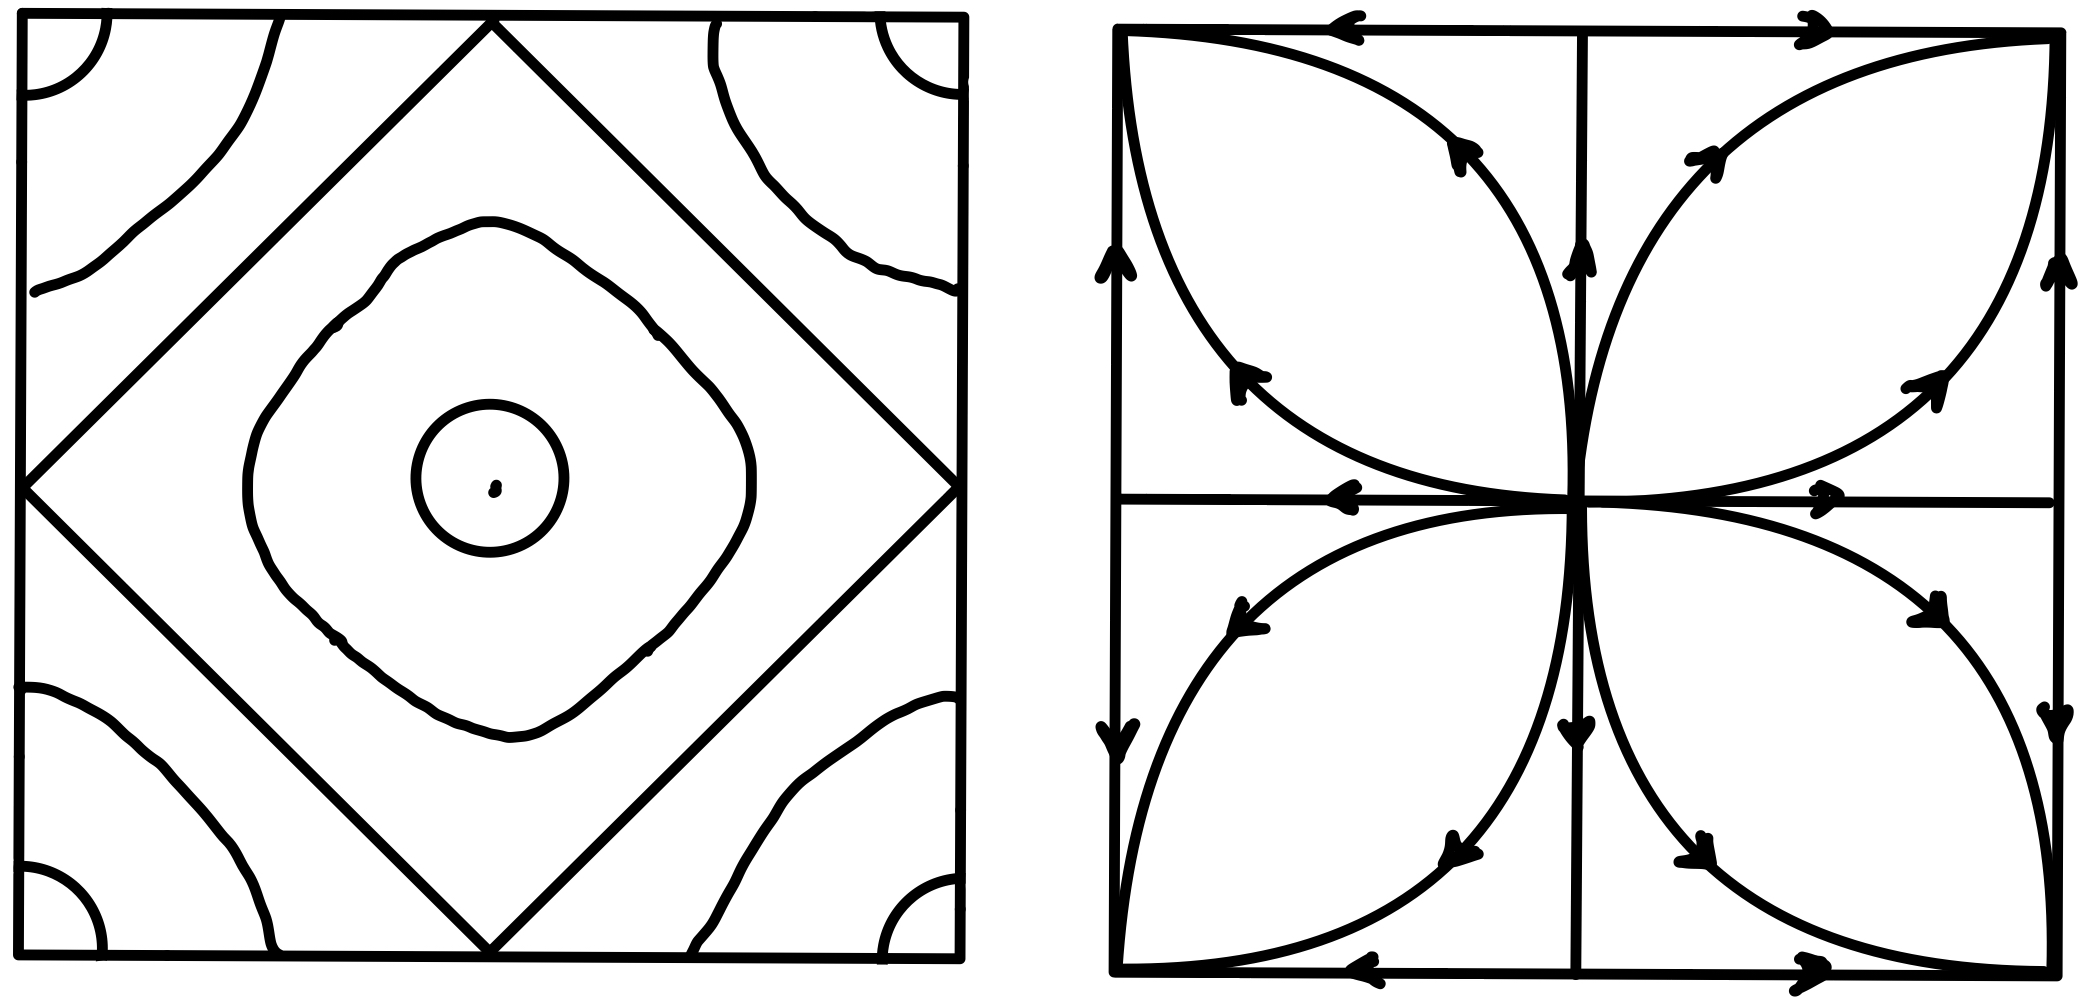
\includegraphics[width=0.4\textwidth]{../resources/morse-funktion-torus.jpeg}
    \end{figure}
    Der Punkt $p = (\sfrac{1}{2}, \sfrac{1}{2})$ ist ewin Maximum, die beiden Punkte 
        $c_1 = (0, \sfrac{1}{2}) = (1, \sfrac{1}{2})$ und $c_2 = (\sfrac{1}{2}, 0) = (\sfrac{1}{2}, 1)$
        sind Sattelpunkte und der Eckpunkt $q$ ist ein Minimum. Von $p$ gehen zwei Trajektorien jeweils
        zu $c_1$ und $c_2$ und von $c_1$ und $c_2$ gehen jeweils zwei Trajektorien zu $q$. Der Morse-
        Komplex ist also der folgende:
        \[ \begin{tikzcd}[row sep=tiny]
            \text{Grad:} & 3 & 2 & 1 & 0 & -1 \\
            & 0 \arrow[r, "0"] & \F_2 \arrow[r, "0"] & \F_2^2 \arrow[r, "0"] & \F^2 \arrow[r, "0"] & 0
        \end{tikzcd} \]
        Dann ist 
        \[ HM_k = \begin{cases}
            0 & \text{ falls } k > 2 \text{ oder } k < 0 \\
            \F_2 & \text{ falls } k = 0 \text{ oder } k = 2 \\
            \F_2^2 & \text{ falls } k = 1
        \end{cases} \]
\end{example}

% \subsection*{Der Morse Komplex über \texorpdfstring{$\Z$}{TEXT}}

% Wir haben nun den Morse Komplex über $\F_2$ definiert. Wir wollen noch allgemeiner einen Komplex
% über $\Z$ definieren. Die meiste Arbeit dafür ist nun schon gemacht. Um den Morse-Komplex über 
% $\Z$ zu definieren, wollen wir den Raum der Trajektorien $\Lt (p, q)$ orientieren. Dafür beschäftigen 
% wir uns ein wenig mit Orientierungen von Vektorräumen.

% \begin{definition}[Orientierung und Koorientierung]
%     Es sei $V$ ein endlich dimensionaler Vektorraum. Seien außerdem $\B_1$ und $\B_2$ Basen von $V$. 
%     Definiere
%     \[ \B_1 \sim_O \B_2 \Longleftrightarrow \det \, _{\B_1}[\id_V]_{B_2} > 0 \]
%     Man rechnet leicht nach dass $\sim_O$ eine Äquivalenzrelation ist und dass es bezüglich $\sim_O$
%     genau zwei Äquivalenzklassen gibt.
%     Zwei Basen heißen \textit{gleich orientiert} wenn sie äquivalent bezüglich $\sim_O$ sind. 
%     Eine \textit{Orientierung} ist eine Wahl der Äquivalenzklasse. Ein \textit{orientierter Vektorraum} 
%     ist ein Vektorraum zusammen mit einer Orientierung. Ist ein Vektorraum orientiert, dann sagen wir 
%     dass eine Basis \textit{positiv orientiert} ist, falls sie gleich orientiert mit der gewählten Basis 
%     ist.

%     Sei nun $U$ ein Unterraum von $V$ und $\B_0$ eine Basis von $U$. Sind $\B_1$ und $\B_2$ Basen von 
%     zwei (möglicherweise verschiedenen) Komplementärräumen von $U$, dann definiere
%     \[ \B_1 \sim_K \B_2 \Longleftrightarrow \det \, _{(\B_1, \B_0)}[\id_V]_{(\B_2, \B_0)} > 0 . \]
%     Man rechnet leicht nach, dass $\sim_K$ eine Äquivalenzrelation ist, dass es bezüglich $\sim_K$
%     genau zwei äquivalenzklassen gibt, und dass $\sim_K$ nicht von der gewählten Basis $\B_0$ abhängt. 
%     Zwei Basen heißen \textit{gleich koorientiert} wenn sie äquivalent sind. Eine \textit{Koorientierung} 
%     von $U$ ist eine Wahl der Äquivalenzklasse. Ein \textit{koorientierter Vektorraum} ist ein Vektorraum 
%     zusammen mit einer Koorientierung. Ist ein Vektorraum koorientiert, dann sagen wir dass eine Basis 
%     eines Komplements von $U$ \textit{positiv koorientiert} ist, falls sie gleich koorientiert mit der 
%     gewählten Basis ist.
% \end{definition}

% \begin{prop}
%     Es seien $U, W \subseteq V$ Untervektorräume, $U$ orientiert und $W$ koorientiert. Dann ist 
%     $U \cap W$ orientiert.
% \end{prop}

% \begin{proof}
%     Wähle eine Basis $\B$ von $U \cap W$. Erweitere $\B$ mit einer positiv koorientierten Basis $\B_1$
%     bezüglich $W$ zu einer Basis von $U$. Dann ist $\B$ positiv orientiert, falls $(\B_1, \B)$ 
%     in $U$ positiv orientiert ist. Dies hängt nicht von der Wahl von $\B_1$ ab:

%     Sei $\B_2$ eine weitere positiv koorientierte Basis eines Komplements von $W$, sodass $(\B_2, \B)$ 
%     eine Basis von $U$ mit derserlben Orientierung wie $(B_1, \B)$ ist. Sei $\tilde{\B}$ gewählt, sodass 
%     $(B, \tilde{\B})$ eine Basis von $W$ ist. Dann sind $(\B_1, \B, \tilde{\B})$ und 
%     $(\B_2, \B, \tilde{\B})$ Basen von $V$, und es gilt
%     \[ 0 < \det \, _{(\B_1, \B, \tilde{\B})}[\id_V]_{(\B_2, \B, \tilde{\B})} = 
%         \det \, _{(\B_1, \B)}[\id_U]_{(\B_2, \B)} \]
% \end{proof}

% \begin{definition}[Orientierung und Koorientierung von Mannigfaltigkeiten]
%     Es sei $M$ eine $n$-dimensionalen Mannigfaltigkeit und 
%     \[ (v_1, \dots, v_n), (w_1, \dots, w_n) \colon M \to TM \times \dots \times TM \]
%     glatte Abbildungen mit $v_i(p), w_i(p) \in T_pM$, für alle $p \in M$ sodass $(v_1(p), \dots, v_n(p))$
%     und $(w_1(p), \dots w_n(p))$ Basen von $T_pM$ sind. Dann definiere:
%     \[ (v_1, \dots, v_n) \sim_O (w_1, \dots, w_n) 
%         \Longleftrightarrow 
%             (v_1(p), \dots, v_n(p)) \sim_O (w_1(p), \dots, w_n(p)) \text{ für alle } p \in M . \]
%     Dies ist wieder eine Äquivalenzrelation und es gibt wieder genau zwei Äquivalenzklassen. 
%     Eine Äquivalenzk
% \end{definition}

% Die stabilen Mannigfaltigkeiten sind offene Kreisscheiben, also offensichtlich orientierbar. 
% Wähle für jeden kritischen Punkt $p$ (endgültig) eine Orientierung von $\stab (p)$. Da gilt 
% $T_p \stab (p) + T_p \unst (p) = T_p M$ und $\dim T_p \stab (p) + \dim T_p \unst(p) = n$,
% gilt schon $T_p \stab (p) \oplus T_p \unst (p) = T_p M$. Die Wahl der Orientierung von $\stab (p)$
% ist also gleichzeitig eine Wahl der Koorientierung von $\unst (p)$. Dann ist für kritische Punkte 
% $\stab (p) \cap \unst (p)$ eine orientierte Mannigfaltigkeit. 

% Bemerke nun, dass fur einen regulären Wert $c$ die Niveau-Menge $f^{-1}(c)$ transversal zum 
% Pseudo-Gradientenfeld $X$ liegt, und da $f^{-1}(c)$ $n-1$-dimensional ist definiert $X$ eine 
% Koorientierung von $f^{-1}(c)$. Außerdem gilt für reguläre Werte mit $f(p) > c > f(q)$, dass 
% $\Lt (p, q) = (\unst (p) \cap \stab (q)) \cap f^{-1}(c)$. Also ist $\Lt (p, q)$ orientiert.

% Falls nun $p$ und $q$ kritische Punkte mit $\Index (p) = \Index (q) + 1$ sind, dann ist wieder 
% $\Lt (p, q)$ nur eine Ansammlung von Punkten, die alle mittels der Orientierung mit einem Vorzeichen 
% ausgestattet wurden. Es sei $N_X (p, q)$ die Summe dieser Vorzeichen. Dann sei $C_k (M, (f, X))$
% das von den kritischen Punkten von $f$ mit Index $k$ erzeugte $\Z$-Modul, und für einen kritischen $p$
% sei
% \[\del_X (p) = \sum_{\substack{ q \in \Crit(f) \\ \Index (p) + 1 = \Index (q) }} N_X(p, q)p . \]

% Wir müssen nun dieselben Fragen beantworten wie für den Komplex über $\F_2$. 

% Offensichtlich ist $N_X(p, q) < \infty$. Wir müssen also noch zeigen, dass gilt
% \[ \del_X \circ \del_X (p) = 0 . \]
% Dies folgt aus dem Satz~\ref{satz: gebrochene trajektorien sind 1-dim mannigfaltigkeit}.
% Die Kompaktifizierung einer orientierten \\ 
% $1$-dimensionalen Mannigfaltigkeit zu einer $1$-dimensionalen 
% Mannigfaltigkeit mit Rand ist offensichtlich wieder orientiert. Wir müssen nur noch sicherstellen, dass 
% die Orientierung auf dem Rand dann auch mit der Orientierung, die wir oben festgelegt haben übereinstimmt.



\chapter{Morse-Homologie und zelluläre Homologie}

In diesem Kapitel wird aus einem Morse-Smale Paar auf einer Mannigfaltigkeit
eine zelluläre Struktur dieser Mannigfaltigkeit konstruiert. Dann werden wir 
sehen, dass der Kettenkomplex, der von dieser Struktur induziert wird schon mit
dem Morse-Komplex übereinstimmt. Somit stimmt die Morse-Homologie mit der 
zellulären Homologie überein, also auch mit der singulären Homologie.

\section{CW-Struktur von Mannigfaltigkeiten}

Die folgenden Definitionen sind in \cite{dold} zu finden.

\begin{definition}[CW-Zerlegung und CW-Komplexe]
    \label{def: cw-komplex}
    Es sei $X$ ein topologischer Raum. Eine offene Überdeckung $\mathcal{E}$ von $X$ heißt 
    $CW-Zerlegung$, wenn gelten:
    \begin{enumerate}
        \item Die Elemente in $\mathcal{E}$ sind paarweise disjunkt.
        \item Alle $e \in \mathcal{E}$ sind homeomorph zu offenen Kreisscheiben. \\
            Wir nennen $X^n$ die Vereinigung aller $e \in \mathcal{E}$, die Homeomorph zu einer
            $k$-dimensionalen offenen Kreisscheibe mit $k \leq n$ sind.
        \item Für jedes Element $e \in \mathcal{E}$ existiert eine stetige Abbildung
            $\Phi_e \colon (B^n, S^{n - 1}) \to (X^n \cup e, X^n)$, sodass 
            $\Phi_e \colon B^n - S^n \to e$ ein Homeomorphismus ist. $B^n$ ist die abgeschlossene 
            $n$-dimiensionale Kresscheibe.
        \item Der Abschluss $\overline{e}$ enthält nur endlich viele Elemente aus $\mathcal{E}$.
        \item Eine Teilmenge $U$ ist offen in $X$ genau dann, wenn für alle $e \in \mathcal{E}$ die
            Menge $U \cap \overline{e}$ offen in $\overline{e}$ ist. 
    \end{enumerate}
    
    Ein topologischer Raum $X$ zusammen mit einer CW-Zerlegung $\mathcal{E}$ heißt 
    \textit{CW-Komplex}.
    Wir nennen die $k$-dimensionalen $e \in \mathcal{E}$ $k$-Zellen, die Abbildung $\Phi_e$
    heißt charakteristische Abbildung von $e$, die Abbildung 
    $\phi_e := \Phi_e|_{S^{n - 1}} \colon S^{n - 1} \to X^{n - 1}$ heißt Anheftungsabbildung.
    $X^n$ heißt $n$-Skelett von $X$. Existiert ein $n$, sodass $X^n = X$, dann ist $n$ die 
    dimension des CW-Komplexes. Existiert kein solchens $n$, dann ist die Dimiension $\infty$.
\end{definition}

\begin{remark}
    Ist $X$ kompakt mit einer CW-Zerlegung $\mathcal{E}$, dann ist $\mathcal{E}$ endlich dimensional, 
    und die Bedingungen 4. und 5. sind sowieso erfüllt.
\end{remark}

\begin{definition}[Zelluläre Homologie]
    \label{def: zellulaere homologie}
    Bemerke, dass $X^n / X^{n - 1}$ das Wedge-Produkt vieler $D^n / S^{n-1} = S^n$'s ist. 
    Wir bekommen durch die Anheftungsabbildung für jede $k$-Zelle $e$ eine Abbildung in den 
    Quotienten
    \[ \phi_e \colon S^{k-1} \longto X^{k - 1} \longto X^{k - 1} / X^{k - 2} . \]
    ist $d$ eine $k - 1$-Zelle, dann bekommen wir außerdem eine Abbildung 
    \[ \psi_d \colon X^{k - 1} / X^{k - 2} \longto S^{k - 1} , \]
    die alle Sphären in dem Quotienten außer die, die aus $\Ima (\Phi_d)$ entstanden ist
    auf den Klebepunkt abbildet.

    Sei dann $N(e, d)$ der Grad$\mod 2$ der Abbildung
    \[ \psi_d \circ \phi_c \colon S^{k - 1} \longto S^{k - 1} . \]
    Dann ist das $k$-te Glied $K_k$ des \textit{zellulären Komplexes} $(K_{\ast}, \del)$ das 
    $\F_2$-Modul, das von den $k$-Zellen in $\mathcal{E}$ erzeugt wird, und das Differential ist für 
    eine $k$-Zelle $e$ gegeben durch
    \[ \del (e) = \sum_{d \in K_{k  - 1}} N(e, d) \cdot d \] 
\end{definition}

\begin{remark}
    Man zeigt, dass $\del \circ \del = 0$, also dass $(K_{\ast}, \del)$ ein Kettenkomplex ist. 
    Siehe \cite{dold}. Außerdem ist die Homologie des zellulären Kettenkomplexes isomorph zur 
    singulären Homologie, und damit unabhängig von der gewählten CW-Zerlegung (\cite{hatcher}). 
    Wie schon vorher angedeutet, gibt es nicht für jeden topologischen Raum eine CW-Zerlegung,
    aber es ist tatsächlich gar nicht leicht einen topologischen Raum zu konstruieren, der 
    kein CW-Komplex ist.
\end{remark}


\section{Morse-Homologie ist zelluläre Homologie}

Das Ziel dieses Abschnittes ist es, mithilfe der im 2. Kapitel erarbeiteten Mitteln eine 
CW-Zerlegung von einer kompakten Mannigfaltigkeit $M$ zu finden.

Wir kennen schon eine disjunkte Zerlegung von $M$ in offene Kreisscheiben, nämlich
\[ \mathcal{E} = \{ \unst (p): p \in \Crit (f) \} . \]
Tatsächlich ist jede instabile Mannigfaltigkeit eine offene Kreisscheibe und jeder Punkt in 
$ p \in M$ wird von $\phi_{\bullet}(p)$ für $t \to - \infty$ genau auf einen kritischen Punkt 
transportiert (siehe Prop.~\ref{prop: trajektorien enden in kritischen punkten}), also ist 
$\mathcal{E}$ eine disjunkte Überdeckung.

\begin{prop}
    \label{prop: cw-zerlegung}
    Die Zerlegung $\mathcal{E} = \{ \unst (p): p \in \Crit (f) \}$ ist eine CW-Zerlegung.
\end{prop}

Bevor wir diese Proposition beweisen können, müssen wir noch ein wenig arbeiten.
Wir definieren für einen kritischen Punkt $p$:
\[ \clunst (p) = 
    \unst (p) \cup \left( \bigcup_{q \in \Crit (f)} \Lb (p, q) \times \unst (q) \right) . \]

$\Lb (p, q) \times \unst (q)$ ist nur nicht leer, wenn $\Index (p) > \Index (q)$.
Für alle $x \in \unst (p) - \{ p \}$ gibt es einen kritischen Punkt $q$ und eine Trajektorie 
$\lambda_x \in \Lt (p, q)$, sodass $x \in \lambda_x$. wir können also jedes 
$x \in \unst (p) - \{ p \}$ künstlich zu einem Tupel $(\lambda_x, x)$ machen. Wir werden im Folgenden
nicht zwischen $x$ und $(\lambda_x, x)$ in $\unst (p)$ unterscheiden.

Wie im letzten Kapitel geben wir für $\clunst (p)$ eine Topologie:

\begin{definition}[Topologie von $\clunst (p)$]
    Wir definieren eine Basis der Topologie von $\clunst (p)$. Offene Mengen in $\unst (p)$ sind 
    auch in $\clunst (p)$ offen. Für $(\lambda, x) \in \Lt (p, c_1) \times \Lt (c_{k - 1}, c)$,
    eine Umgebung $U^0$ von $x$ in $M$ und $U^+$ und $U^-$ wie vorher 
    in~\ref{def: topologie gebrochener trajektorien} die Vereinigungen offener Umgebungen der Ein-
    bzw. Austrittspunkte der jeweiligen Trajektorien in $\del_+ \Omega (c_i)$ bzw. 
    $\del_- \Omega (c_i)$ definieren wir die restlichen Elemente 
    $\mathcal{U}(\lambda, x, U^0, U^-, U^+)$ der Basis
    wie folgt: \\
    Falls $(\mu, x') \in \Lb(p, c_i) \times \unst (c_i)$ oder $(\mu, x') \in W^u (p) \cap \stab (c)$, 
    dann ist \[ (\mu, x') \in \mathcal{U}(x, \lambda, U^0, U^-, U^+) , \]
    falls gelten:
    \begin{enumerate}
        \item $x' \in U^0$.
        \item Die (einfache) Trajektorie, die $c_i$ mit $x'$ verbindet, tritt in $\Omega (c_j)$ durch 
            $U^+_j$ für alle $j > i$ und verlässt $\Omega (c_j)$ durch $U^-_j$ für alle $j \geq i$.
            Eine solche Trajektorie existiert, da $x' \in \unst (c_i)$.
        \item $\mu \in \mathcal{U}(\tilde{\lambda}, \tilde{U}^-, \tilde{U}^+)$, wobei 
            $\tilde{\lambda} = (\lambda_1, \dots, \lambda_i)$ und 
            $\tilde{U}^{\pm} = \bigcup_{j = 1}^i U^{\pm}_j$
    \end{enumerate}
    Für $(\mu, x) \in \unst(p) \cap \stab (c)$ sind die zweite und die dritte Bedingung äquivalent.
    Die offenen Mengen in $\clunst (p)$ sind dann die Mengen, die sich als Vereinigung der 
    Elemente der Basis schreiben lassen. 
\end{definition}

\begin{example}
    \begin{itemize}
        \item Die Höhenfunktion $f$ von $S^2 \subseteq \R^3$ ist eine Morse Funktion. Diese hat 
            zwei kritische Punkte: den Nordpol $n$ und den Südpol $s$. Es gilt 
            $\unst (n) = S^2 - \{ s \}$ und $\unst (s) = \{ s \}$. $\Lb (n, s) = \Lt (n, s) = S^1$,
            und dann ist $\clunst (n)$ die abgeschlossene Kreisscheibe mit Rand $\Lt (n, s)$. 
        \item Wir betrachten den kritischen Punkt $p$:
            \begin{figure}[H]
                \centering
                \begin{tikzpicture}
                    % Include the image in a node
                    \node [
                        above right,
                        inner sep=0] (image) at (0,0) {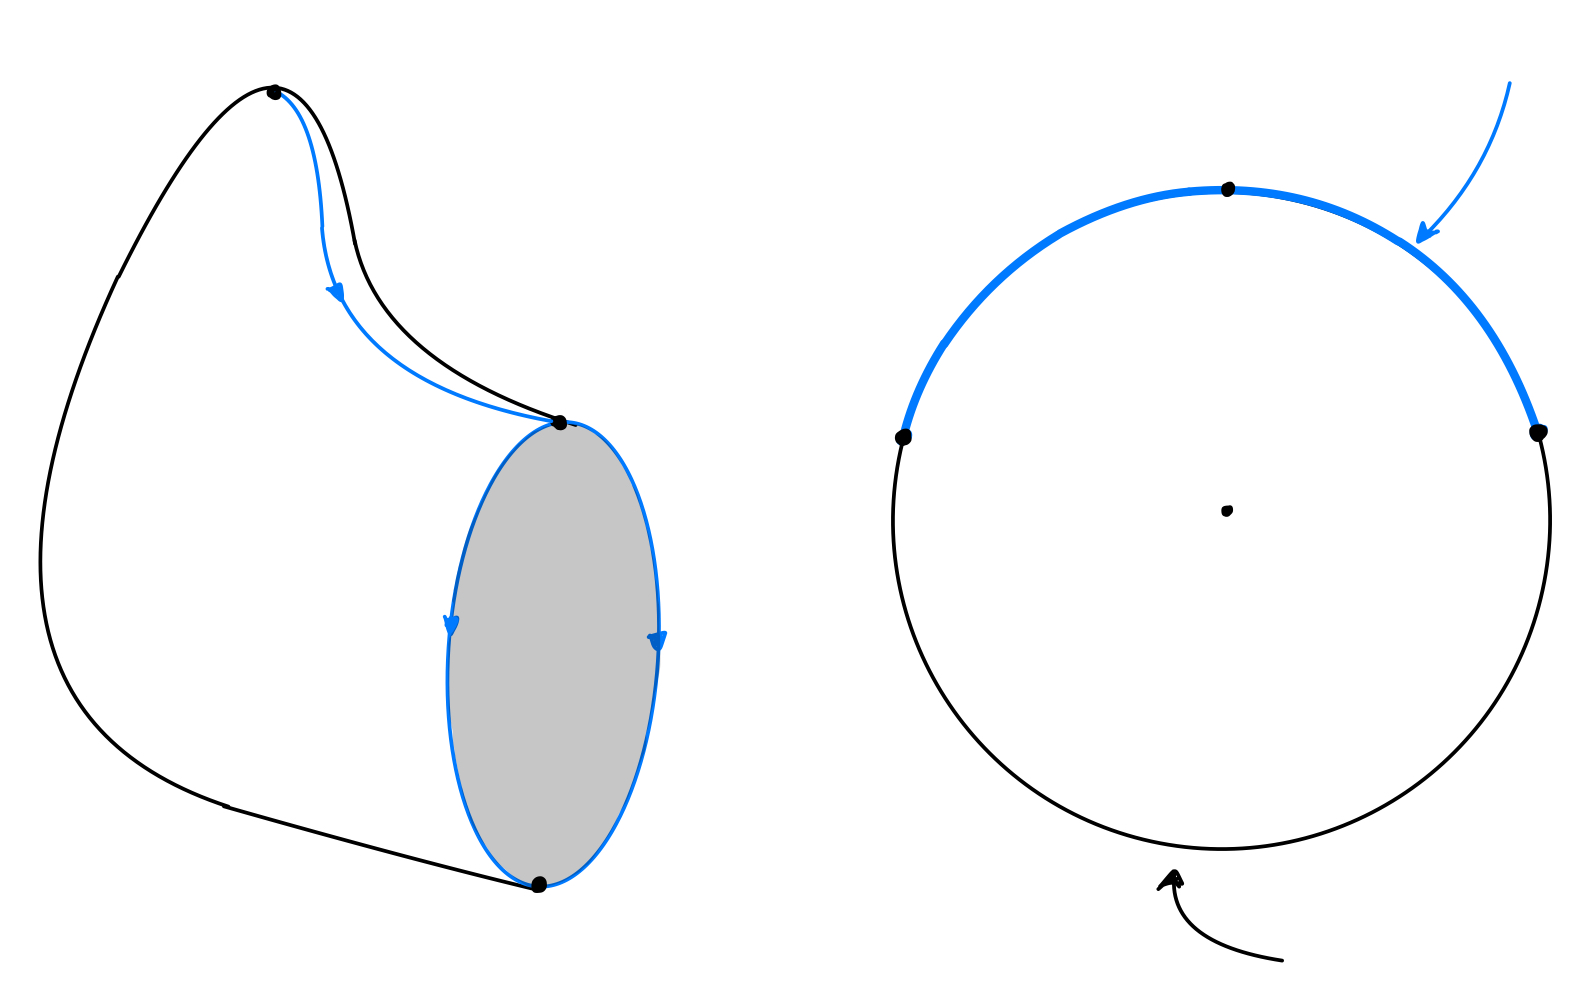
\includegraphics[width=0.4\textwidth]{../resources/clunst-beispiel.jpeg}};
                        
                    % Create scope with normalized axes
                    \begin{scope}[
                    x={($0.05*(image.south east)$)},
                    y={($0.1*(image.north west)$)}]

                    % Annotate left figure
                    \node at (3.5, 9.5) {\tiny $p$};
                    \node at (7, 6.2) {\tiny $c$};
                    \node at (7, 0.6) {\tiny $q$};
                    
                    \node[text=LightBlue] at (4.2, 6.2) {\tiny $\ell$};
                    \node[text=LightBlue] at (5, 3.8) {\tiny $\ell_1$};
                    \node[text=LightBlue] at (9, 3.8) {\tiny $\ell_2$};

                    % Annotaste right figure
                    \node at (15.5, 4.5) {\tiny $p$};
                    \node at (15.5, 8.5) {\tiny $(\ell, c)$};

                    \node at (13.3, 5.6) {\tiny $((\ell, \ell_1), q)$};
                    \node[right] at (19.1, 5.6) {\tiny $((\ell, \ell_1), q)$};

                    \node at (19, 0.5) {\tiny $\Lb (p, q) \times \{ q \}$};
                    \node[text=LightBlue] at (19, 9.5) {\tiny $\{ \ell \} \times \unst (c)$};

                    % \draw[lightgray,step=1] (image.south west) grid (image.north east);
                    \end{scope}
                \end{tikzpicture}
            \end{figure}
    \end{itemize}
\end{example}

\begin{prop}
    \label{prop: abschluss von instabilen mannigfaltigkeiten}
    Ist $p$ ein kritischer Punkt von $f$, $k = \Index (p)$, dann ist $\clunst (p)$ homeomorph 
    zur abgeschlossenen Kreisscheibe $D^k$, und $\unst (p)$ ist das Innere von $\clunst (p)$.
\end{prop}

\begin{remark}
    Mit dieser Proposition wird auch Proposition~\ref{prop: cw-zerlegung} bewiesen:
    Die ersten beiden Bedingungen für CW-Zerlegungen sind schon erfüllt. Da wir annehmen, dass 
    $M$ kompakt ist, sind auch die letzten beiden Bedingungen erfüllt. Die dritte Bedingung folgt
    dann sofort aus der letzten Proposition~\ref{prop: abschluss von instabilen mannigfaltigkeiten}.
\end{remark}

\begin{bigproof}
    Wir geben nur eine grobe Beweisidee. Den detaillierten Beweis findet man in \cite{audin}.
    Für Elemente $(\lambda, x) \in \clunst (p)$ gilt sowieso schon, dass $f(x) \leq f(p)$. Definiere
    \[ \clunst (p, \alpha) = 
        \{ (\lambda, x) \in \clunst (p) - \{ p \} : f(x) \geq \alpha \}  \cup \{ p \} . \]
    Für $\alpha = f(c) - \eps$ und $\eps$ klein genug gilt 
    \[ \clunst (p, \alpha) = \unst (p) \cap \Omega (p, \eps, \eta) . \]
    Für ein beliebiges $\eta$. $\Omega (p, \eps, \eta)$ ist wie in der Notation zu 
    Morse-Umgebungen~\ref{def: notation morse umgebung}. Dies ist via einer Morse-Karte homeomorph 
    zu $V^- \cap U(\eps, \eta)$, also zur abgeschlossenen $\Index (p)$-dimensionalen Kreisscheibe.
    Da $M$ kompakt ist besitzt $f$ ein Minimum, und falls gilt $\alpha < \min (f)$, dann gilt 
    offenbar
    \[ \clunst (p, \alpha) = \clunst (p) . \]
    Wir wollen also zeigen, dass für $\alpha' < \alpha$ gilt
    \[ \clunst (p, \alpha') \isom \clunst (p, \alpha) . \]
    Die Menge $\clunst (p, \alpha)$ erinnert uns an die Subniveaumengen aus 
    Abschnitt~\ref{sec: topologische eigenschaften anhand kritischer punkte}. Das erste 
    Deformationslemma liefert eine ähnliche Aussage, und wir können die folgende Behauptung 
    beweisen:

    \begin{claim}
        Wenn sich im Intervall $[\alpha', \alpha]$ keine kritischen Werte von $f$
        befinden, dann sind $\clunst (p, \alpha')$ und $\clunst (p, \alpha)$ homeomorph.
    \end{claim}

    \begin{smallproof}
        Unter Anwendung des ersten Deformationslemmas auf $-f$ bekommen wir einen Homeomorphismus
        \[ \phi \colon M^{\alpha'} \longto M^{\alpha} . \]
        Die Subniveaumengen sind die Subniveaumengen von $-f$. Dann ist auch 
        \begin{align*}
            \chi \colon \clunst (p, \alpha') \longto & \clunst (p, \alpha) \\
            (\lambda, x) \longmapsto & (\lambda, \phi(x))
        \end{align*}
        ein Homeomorphismus.
    \end{smallproof}

    Sehr viel schwieriger ist es zu beweisen, dass sich $\clunst (p, \alpha)$ selbst wenn $\alpha$
    einen kritischen Wert überquert nicht verändert. Für den Fall $\Index (p) = \Index (q) + 1$
    und $\Index (q) \neq 0$ liefert die folgende Skizze eine Idee für den Beweis:

    \begin{figure}[H]
        \label{fig: definition von chi}
        \centering
        \begin{tikzpicture}
            % Include the image in a node
            \node [
                above right,
                inner sep=0] (image) at (0,0) {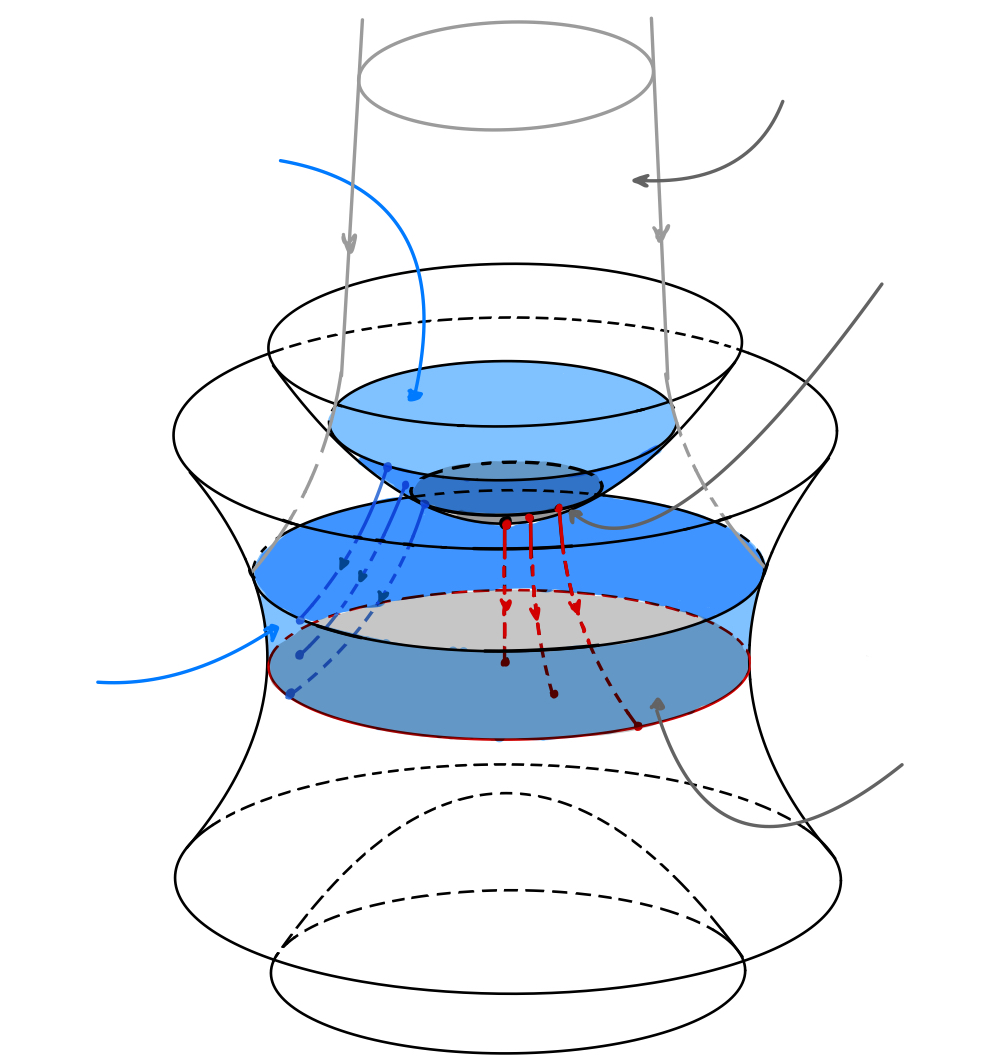
\includegraphics[width=0.4\textwidth]{../resources/cw-zerlegung.jpeg}};
                
            % Create scope with normalized axes
            \begin{scope}[
            x={($0.05*(image.south east)$)},
            y={($0.05*(image.north west)$)}]

            \node[text=LightBlue] at (0, 7) {\small $\Ima (\Phi)$};
            \node[text=DarkGray] at (22, 6.4) {\small $\unst (c) \cap f^{-1}[\alpha - \eps, \infty)$};
            \node[text=DarkGray] at (18.5, 15.2) {\small $B'$};
            \node[text=LightBlue] at (3.5, 17) {\small $B - B'$};
            \node[text=DarkGray] at (15.7, 18.8) {\small $U$};

            % \draw[lightgray,step=1] (image.south west) grid (image.north east);
            \end{scope}
        \end{tikzpicture}
        \caption{Definition von $\chi$}
    \end{figure}
    
    Wir nehmen an, dass es für jeden kritischen Wert $\alpha$ genau einen kritischen Punkt $c$ gibt, 
    sodass $f (c) = \alpha$. Es sei $c$ ein weiterer kritischer Punkt mit $f(c) = \alpha$. Dann sei $\eps > 0$, 
    sodass sich im Intervall $f^{-1}[\alpha - \eps, \alpha + \eps]$ keine kritischen Punkte außer $c$ befinden.
    Wir bekommen in diesem Fall nur ein Problem, wenn wir einen Punkt $x$ haben, der von seiner Trajektorie 
    auf den kritischen Punkt $c$ geschickt wird - ansonsten können wir wie im Beweis von Behauptung 1
    den Punkt $x$ entlang seiner Trajektorie entlang des (skalierten) Pseudo-Gradientenfeldes nach unten ziehen. 
    Wir definieren also
    \[ P = \{ (x, \lambda) \in \clunst (p, \alpha + \eps) : x \in \unst (c) \} . \]
    Außerhalb von einer Umgebung von $P$ können wir 
    \[ \chi \colon \clunst (p, \alpha + \eps) \longto \clunst (p, \alpha - \eps) \]
    wie in Behauptung 1 angedeutet definieren.

   Wir zeigen dies nur für den einfachsten Fall:

    \begin{claim}
        Ist $\alpha = f(p)$, $q$ ein weiterer kritischer Punkt von $f$ mit 
        $\Index (p) = \Index (q) + 1 \neq 0$ und $\eps > 0$ klein genug, dann sind 
        $\clunst (p, \alpha + \eps)$ und $\clunst (p, \alpha - \eps)$ homeomorph.
    \end{claim}

    \begin{smallproof}
        In diesem Fall gilt 
        \[ P \subseteq \mathcal{M} (p, c) \subseteq \unst (p) \subseteq \clunst (p) \]
        Der Beweis erinnert an den Beweis von Satz~\ref{satz: gebrochene trajektorien sind 1-dim mannigfaltigkeit}.
        Man betrachte die Folgende Abbildung:

        Da der Index sich nur um $1$ unterscheidet ist $\Lb (p, c) = \Lt (p, c)$ eine endliche Ansammlung 
        von Trajektorien. Für jede dieser Trajektorien $\ell$ wähle eine Umgebung wie in 
        Fig.~\ref{fig: definition von chi} angedeutet:

        Die Umgebung von $P$ ist an den Seiten von den äußeren Trajektorien begrenzt und oben und unten von den
        Niveaumengen $f^{-1}(\alpha + \eps + \delta)$ und $f^{-1}(\alpha - \eps)$. Wir finden wie im Beweis 
        von Satz~\ref{satz: gebrochene trajektorien sind 1-dim mannigfaltigkeit} eine Kreisscheibe 
        $B \subseteq f^{-1}(\alpha + \eps) \cap \unst (p)$, die transversal zu $S_+(c)$ ist, vollständig in der 
        gewählten Umgebung von $P$ enthalten ist und eine Umgebung vom Schnittpunkt 
        $\ell \cap f^{-1}(\alpha + \eps)$ ist. Die existenz solcher Umgebungen transversal zu $S_+(c)$ folgt 
        aus der Smale-Bedingung. Außerdem wählen wir eine weitere kleinere Kreisscheibe $B'$, 
        die die selben Eigenschaften wie $B$ und sodass gilt $B' \subsetneq B$. 

        Die graue Scheibe in der Mitte vom Bild ist $\unst (c) \cap f^{-1} [\alpha - \eps, \infty)$. 
        Wir identifizieren diese Kreisscheibe mit 
        \[ \{ \ell \} \times \unst (c) \cap f^{-1} [\alpha - \eps, \infty) \subseteq 
            \clunst (c, \alpha - \eps) . \]
        Wenn wir unsere Umgebung nun entlang der angedeuteten Pfeile ähnlich wie im Beweis 
        von~\ref{satz: erstes deformationslemma} \say{nach unten ziehen}, sodass 
        $B - B'$ auf den gefärbten Zylinderabschnitt $\Ima (\Phi)$ und $B'$ auf die mittlere Kreisscheibe 
        abgebildet wird. $\Phi$ ist wie im Beweis 
        von~\ref{satz: gebrochene trajektorien sind 1-dim mannigfaltigkeit}. 
        Es ist möglich diese Abbildung so zu wählen, dass sie am Rand der Umgebung der 
        oben gewählten Abbildung entspricht und dass es ein Homeomorphismus ist.
    \end{smallproof}

    Für einen beliebigen kritischen Punkt $c$ funktioniert der Beweis ähnlich.
\end{bigproof}

\begin{theorem}[Morse-Homologie ist zelluläre Homologie]
    \label{satz: morse-homologie ist zellulaere homologie}
    Es existiert eine Isomorphie von Kettenkomplexen zwischen dem zelluläre Kettenkomplex 
    $(C^{Cell}(X, \mathcal{E})_{\ast}, \del)$, der durch die CW-Zerlegung in instabilen 
    Mannigfaltigkeiten durch 
    Proposition~\ref{prop: cw-zerlegung} gegeben ist, und dem Morse-Komplex 
    $(C_{\ast}(M, (f, X)), \del_X)$.
\end{theorem}

\begin{proof}
    Es sei $F \colon C_k (M, (f, X)) \to C^{Cell}(X, \mathcal{E})$ die lineare Abbildung, 
    die den kritischen Punkt $p$
    auf die Zelle $\unst (p)$ schickt. Dann bildet $F$ Erzeuger auf Erzeuger ab, ist also 
    offensichtlich ein linearer Isomorphismus. Wir wollen zeigen, dass 
    $F \circ \del_X = \del \circ F$. Wir zeigen sogar, dass für kritische Punkte $p$ und $q$ mit 
    Index $k$ und $k - 1$ die Zahl $N (\unst (p), \unst (q))$, also der Grad der Abbildung 
    $\psi_{\unst (q)} \circ \phi_{\unst (p)}$ modulo $2$ gleich der Zahl $n_X(p, q)$, also 
    der Anzahl der Trajektorien von $p$ nach $q$ modulo $2$ ist. 

    Da $\Lt (p, q)$ $0$-dimensional ist, gilt $\Lb (p, q) = \Lt (p, q)$ und dann befinden sich im 
    Rand von $\clunst (p)$, also 
    \[ \bigcup_{c \in \Crit (f)} \Lb (p, c) \times \unst (c) \isom S^{k - 1} , \] 
    genau $\# \Lt (p, q)$ disjunkte Kopien von $\unst (q) \isom B^{k - 1}$. Jede dieser Kopien 
    wird mit der Anbringungsabbildung $\phi_{\unst (p)}$ via der Inklusion auf die Zelle $\unst (q)$
    geschickt. Wenn wir nun $M$ mit der Abbildung $\psi_{\unst (q)}$ kollabieren, dann ist 
    $\psi_{\unst (q)} (M)$ die $1$-Punkt-Kompaktifizierung von $\unst (q)$ und 
    \[ \phi_{\unst (p)} \circ \psi_{\unst (q)} |_{ \{ \lambda \} \times \unst (q) } \]
    Ist die Inklusion von $\unst (q)$ in ihre $1$-Punkt-Kompaktifizierung. Wir wissen, dass 
    $\unst (q) \isom B^{k - 1}$, und dass die Kopien $\{ \ell \} \times \unst (q)$ in 
    $\del \clunst (p)$ disjunkt sind, wir haben also die folgende Situation:
    Eine stetige Abbildung $\Phi \colon S^{k - 1} \to S^{k - 1}$, endlich viele disjunkte Kopien 
    $(\ell, B^{k - 1}) \subseteq S^{k - 1}$, sodass ein Punkt $\ast$ in $S^{k - 1}$ existiert, sodass
    \[ \Phi \colon (\ell, B^{k - 1}) \to S^{k - 1} - \{ \ast \} \]
    für jedes $\ell$ ein Homeomorphismus ist und sodass
    \[ \Phi \left( S^{k - 1} - \bigcup_{\ell} \left( \ell, B^{k - 1} \right) \right) = \{ \ast \} . \]
    Es sei $m$ die Anzahl der Kopien von $B^{k - 1}$ in $S^{k - 1}$
    Wir benutzen die lokale Grad Formel (siehe zum Beispiel \cite{hatcher}): 
    
    Wähle einen von $\ast$ verschiedenen Punkt $y$ in $S^{k - 1}$. Dann ist 
    $\Phi^{-1}(y) = \{ x_{\ell} \}_{\ell}$ mit $x_{\ell} \in (\ell, B^k)$. 
    $\Phi \colon (\ell, B^k) \to S^{k - 1} - \{ \ast \}$ ist ein Homeomorphismus, also ist 
    \[ \Phi_{\ast} \colon H_{k - 1} ((\ell, B^{k - 1}), (\ell, B^{k - 1}) - x_{\ell}) \to 
        H_{k - 1}(S^{k - 1} - \{ \ast \}, S^{k - 1} - \{ \ast, y \}) \]
    ein Isomorphismus, dann sind alle lokalen Grade $1$ oder $-1$. Dann ist 
    \[ \deg \Phi = \sum_{\ell} (\pm_{\ell} 1) = m \mod 2 \]
    Damit ist die Aussage gezeigt.
\end{proof}

Zum Beispiel bei Hatcher \cite{hatcher} kann man nachlesen, wie für einen topologischen Raum die 
singuläre Homologie $H_{\ast} (X)$ definiert wird. Insbesondere hängt diese nur vom topologischen 
$X$ Raum ab. Hatcher zeigt auch: 

\begin{theorem}
    \label{satz: zellulaere Homologie ist singuläre Homologie}
    Für jedes $k \in \N$ gilt 
    \[ H_k (X) \isom HC_k (X, \mathcal{E}) . \]
\end{theorem}

Die zelluläre Homologie ist also nicht von der gewählten CW-Zerlegung abhängig und wir können schreiben
\[ HC_{\ast} (X) := HC_{\ast} (X, \mathcal{E}) \]

Da aber für eine kompakte Mannigfaltigkeit $M$ und ein Morse-Smale Paar $(f, X)$ gilt 
\[ HM_k(M, (f, X)) \isom HC_k(X) , \]
folgt direkt:

\begin{theorem}
    Die Morse-Homologie ist nicht vom gewählten Morse-Smale Paar abhängig, und wir können schreiben
    \[ HM_{\ast} (M) := HM_{\ast}(M, (f, X)) \]
\end{theorem}

\section{Anwendungen}

Die berühmten Morse Ungleichungen lassen sich, wie am Ende des ersten Kapitels erwähnt, sehr
leicht aus den Eigenschaften der Morse-Homologie folgern. Außerdem sind einige bekannten 
Eigenschaften singulärer Homologie sofort ersichtlich.

\begin{theorem}[Die Morse-Ungleichungen]
    \label{satz: morse-ungleichungen}
    Es sei $M$ eine kompakte Mannigfaltigkeit und $f$ ein Morse-Funktion auf $M$.
    Wir definieren:
    \begin{itemize}
        \item $\betti_k (M) := \dim HM_k (M)$ ist die $k$-te Betti-Zahl.
        \item $\chi(M) := \sum_k (-1)^k \cdot \betti_k(M)$ ist die Euler-Charakteristik.
        \item $C_k$ ist die Anzahl der kritischen Punkte von $f$ mit Index $k$.
    \end{itemize}
    Dann gelten die folgenden Ungleichungen:
    \begin{enumerate}
        \item $\betti_k(M) - \betti_{k - 1}(M) + \dots \pm \betti_0(M) \leq
            C_k - C_{k - 1} + \dots \pm C_0$
        \item $\chi (M) = \sum_k (-1)^k \cdot C_k$
        \item $\betti_k(M) \leq C_k$
    \end{enumerate}
    3. ist die so genannte \emph{schwache} Morse-Unkgleichung, denn sie folgt direkt aus 1.
\end{theorem}

\begin{proof}
    Es sei $X$ ein Pseudogradientenfeld welches die Smale Bedingung erfüllt.

    2. Ist ein bekanntes Ergebnis über Kettenkomplexe, denn $C_k = \dim(C_k (M, (f, X)))$,

    1. Folgt sofort,

    3. folgt aus 1.:

    Subtrahiere die Ungleichung 1., bei der wir für $k$ die Zahl $k - 1$ einsetzten von der 
    Ungleichung 1.
\end{proof}

\begin{theorem}[Poincaré-Dualität]
    \label{satz: poincare-dualität}
    Es sei $M$ eine komapkte $n$-dimensionale Mannigfaltigkeit ohne Rand. Dann gilt für alle 
    $k \in \{ 0, \dots, n\}$:
    \[ HM_k (M) \isom HM_{n - k} (M) \]
\end{theorem}

\begin{proof}
    Es sei $(f, X)$ ein Morse-Smale Paar. Die kritischen Punkte von $f$ mit Index $k$ sind kritische Punkte
    von $-f$ mit Index $n - k$, und $-X$ ist ein Pseudo-Gradientenfeld von $-f$. Die kritischen Punkte 
    $p$ mit Index $k$ bilden eine Basis von $C_k (M, (f, X))$ und auch von $C_{n - k}(M, (-f, -X))$.
    Es sei $a^{\ast}$ das duale Element von $a$, dann können wir auch $a^{\ast}$ als Basis von 
    $C_{n - k}(M, (-f, -X))$ wählen. Dann gilt $C_{n - k} (M, (-f, -X)) = (C_k (M, (f, X)))^{\ast}$,
    und per Definition ist dann das Differential im Kettenkomplex von $-f$ ist gegeben durch die duale Abbildung
    \[ \del_X^{\ast} \colon C_{n - k} (M, (-f, -X)) \longto C_{n - k - 1} (M, (-f, -X)) . \]
    Es folgt die Behauptung.
\end{proof}


% \appendix

% \chapter{Anhang}

\begin{definition}[Mannigfaltigkeit \cite{ludwig}]
    \label{anh.def: mannigfaltigkeit}
    Es sei $M$ ein topologischer Raum. 
    
    Eine \textit{Karte} von $M$ ist ein Tupel
    $(U, \phi)$, wobei $U \subseteq M$ offen und $\phi \colon U \to U' \in \R^n$ 
    ein Homeomorphismus ist.

    $\mathcal{A} = \left\{ (U_{\alpha}, \phi_{\alpha}) \right\}_{\alpha \in I}$ ist ein 
    \textit{$n$-dimensionaler Atlas} von $M$ falls
    \begin{enumerate}
        \item $(U_{\alpha}, \phi_{\alpha})$ ist eine Karte für jedes $\alpha \in I$
        \item $M = \bigcup_{\alpha \in I U_{\alpha}}$
    \end{enumerate}
    Ein Atlas ist $C^k$ für $k \in \{ \N_0 \cup \{ \infty, \omega \} \}$, falls für
    alle $\alpha, \beta \in I$ der \textit{Koordinatenwechsel} 
    \[ 
        \phi_{\alpha \beta} := 
        \phi_{\alpha} \circ \phi_{\beta}^{-1} \colon 
        \phi_{\beta} (U_{\alpha} \cap U_{\beta}) \to \phi_{\alpha} (U_{\alpha} \cap U_{\beta})
    \]
    $C^k$ ist.
    
    Eine Karte $(U, \phi)$ heißt \textit{$C^k$ kompatibel} mit einem $C^k$ Atlas 
    $\mathcal{A} = \left\{ (U_{\alpha}, \phi_{\alpha}) \right\}_{\alpha \in I}$,
    falls für alle $\alpha \in I$ die Koordinatenwechsel $\phi \circ \phi_{\alpha}^{-1}$
    und $\phi_{\alpha} \circ \phi^{-1}$ $C^k$ sind.

    Eine \textit{$n$-dimensionale $C^k$ Mannigfaltigkeit} ist ein topologischer Raum $M$ 
    zusammen mit einem maximalen $C^k$ Atlas $\mathcal{A}$, sodass $M$ ein Hausdorff-Raum und
    zweitabzählbar ist. Maximal bedeutet hier, dass es keine mit $\mathcal{A}$ $C^k$ 
    kompatiblen Karten gibt, die nicht in $\mathcal{A}$ enthalten sind.

    Eine Mannigfaltigkeit heißt \textit{glatt} falls $k = \infty$.

    Für einen Punkt $p \in M$ und eine Karte $(\phi, U)$ mit $p \in U$ 
    heißen $\phi = (x_1, ..., x_n)$ \textit{lokale Koordinaten} um $p$.
\end{definition}

\begin{remark}
    Wenn der Atlas einer Mannigfaltigkeit angegeben wird, dann nie als maximaler Atlas.
    Es reicht ein Atlas, alle anderen Karten sind dann schon impliziert.
\end{remark}

\begin{definition}[Differenzierbarkeit]
    \label{anh.def: differenzierbarkeit}
    Sind $M, N$ $C^k$ Mannigfaltigkeiten, \\ 
    $\mathcal{A} = (\phi_{\alpha}, U_{\alpha})_{\alpha \in I}$ ein Atlas von $M$, 
    $\mathcal{B} = (\phi_{\beta}, U_{\beta})_{\beta \in J}$ ein Atlas von $N$,
    dann heißt eine Abbildung $C^k$ oder \textit{$k$-mal differenzierbar}, falls für alle 
    $\alpha \in I$ und $\beta \in J$ die Abbildung
    \[ \psi_{\beta} \circ f \circ \phi_{\alpha}^{-1} \colon \R^n \to \R^m \]
    $C^k$ ist.
\end{definition}

\begin{definition}[Tangentialraum]
    \label{anh.def: tangentialraum}
    Der Tangentialraum einer $C^k$ Mannigfaltigkeit $M$ an einem Punkt $p \in M$ ist
    \[ T_pM := \left\{ X_p \colon C^{k} \to \R : X_p 
        \text{ ist eine Derivation von $M$ an dem Punkt $p$} \right\} \]
    Wobei $X_p: C^{k} \to \R$ ein \textit{Derivation} ist, falls folgende Bedingungen erfüllt
    sind:
    \begin{itemize}
        \item $X_p$ ist linear
        \item Für $X_p$ gilt die Leibnitz-Regel, also
            \[ X_p (f \cdot g) = X_p (f) \cdot g + f \cdot X_p (g) \]
    \end{itemize}
    Dann ist $T_pM$ ein Untervektorraum von $C^k(C^k(M))$.

    Für eine $C^k$ Abbildung $f \colon M \to N$  und einen Punkt $p \in M$ ist dann 
    \begin{align*}
        \opd f (p) \colon T_pM & \to T_{f(p)}N \\
        X_p & \mapsto f_* X_p
    \end{align*}
    wobei $f_*X_p$ definiert ist durch
    \[ f_*X_p (g) = X_p (g \circ f) \]
\end{definition}

\begin{remark}
    \begin{align*}
        T \colon \mathbf{Man}_{*} & \to \mathbf{Vect}_{\R} \\
        (M, p) & \mapsto T_pM \\
        f & \mapsto \opd f (p)
    \end{align*}
    Ist ein Funktor.
\end{remark}

\begin{remark}
    Es sei $M$ eine $C^k$ Mannigfaltigkeit, $k \geq 1$, $p \in M$ und $\phi = (x_1, ..., x_n)$
    lokale Koordinaten um $p$. Definiere
    \begin{align*} 
        \pderive{x_1}(p): C^k(M) & \to \R \\
        \pderive[f]{x_i} (p) & = \pderive[\phi \circ f]{x_i} (\phi(p))
    \end{align*}
    Dann ist $\left( \pderive{x_i} \right)_{1 \leq i \leq n}$ eine Basis von $T_pM$.

    Für eine glatte Abbildung $f \colon M \to N$, einem Punkt $p \in M$ und lokale Koordinaten 
    $(x_1, ..., x_n)$ um $p$ und $(y_1, ..., y_m)$ um $f(p)$ bekommen wir in einer Umgebung 
    von $p$ wohldefinierte Abbildungen $f_i = y_i \circ f$. Dann ist das differential 
    $\opd f (p)$ von $f$ gegeben durch die Matrix
    \[ D_p(f) = \left( \pderive[f_i]{x_j} \right)_{i,j} . \]
\end{remark}

\begin{definition}
    \label{anh.def: kritischer punkt}
    Es seien $M, N$ $C^k$ Mannigfaltigkeiten. Sei $f \colon M \to N$ $C^k$. Dann ist $p \in M$
    ein kritischer Punkt von $f$, falls $\opd f (p)$ nicht surjektiv ist. $f(p)$ heißt dann
    kritischer Wert von $f$.
\end{definition}

\begin{theorem}[Whitney's Einbettungssatz, \cite{hirsch}]
    \label{anh.satz: whitneys einbettungssatz}
    Es sei $M$ eine $n$-dimensionale kompakte \todo{Finde eine Quelle ohne Kompaktheit} 
    $C^r$ Mannigfaltigkeit. Dann existiert eine $C^r$ Einbettung von $M$ in 
    $\R^{2n + 1}$.
\end{theorem}

\begin{remark}
    Man kann zeigen, dass jede Mannigfaltigkeit sogar in den $\R^{2n}$ eingebettet werden.
    Diese Version des Satzes heißt \textit{starker Whitney's Einbettungssatz}.
\end{remark}

\begin{theorem}[Satz von Sard (siehe \cite{sard})]
    \label{satz: satz von sard}
    Es seien $M$ und $N$ mindestens \\ 
    $C^q$-Mannigfaltigkeiten mit Dimension $m$ und $n$ respektive
    und $f \colon : \to N$ mindestens $C^q$. Dann gelten:
    \begin{itemize}
        \item Falls $m \leq n$, dann hat die Menge der kritischen Werte von $f$ Maß $0$.
        \item Falls $m > n$, dann hat die Menge der kritischen Werte von $f$ Maß $0$, \\
            falls $q \geq m - n + 1$.
    \end{itemize}
\end{theorem}


\printbibliography

\eject
\end{document}